%% TITLE
%\input{structure/title-page}
%\input{helpers/empty-page}
%\addtocounter{page}{-1}

%% Declaration
%\newpage
%\chapter*{Declaration of Authorship}
%\thispagestyle{empty}
%% !TEX encoding = UTF-8 Unicode
\vspace*{1cm}

\large
\noindent
\IfLanguageName{ngerman}
{Ich versichere, dass ich die vorliegende Arbeit ohne fremde Hilfe und ohne Benutzung anderer als der angegebenen Quellen angefertigt \nobreak habe, und dass die Arbeit in gleicher oder \"ahnlicher Form noch keiner anderen Pr\"ufungsbeh\"orde vorgelegen hat und von dieser als Teil einer Pr\"ufungsleistung angenommen wurde. Alle Ausf\"uhrungen, die w\"ortlich oder sinngem\"a\s{} übernommen wurden, sind als solche gekennzeichnet.}
{I assure that I have produced the present work without the help of others and without using any sources other than those specified and that the work has not been submitted in the same or similar form to any other examination body and has been accepted as part of an examination. All statements, which have been taken literally or meaningfully, are marked as such.}
\vspace{3cm}

\begin{minipage}{0.45\textwidth}
	------------------------------------
	
	\IfLanguageName{ngerman}{Ort, Datum}{Location, Date}
	
\end{minipage}
\begin{minipage}{0.45\textwidth}
	------------------------------------
	
	\IfLanguageName{ngerman}{Unterschrift}{Signature}

	
\end{minipage}

\normalsize
%\pagenumbering{Roman}
%\input{helpers/empty-page}
%\thispagestyle{empty}
%\cleardoublepage

% Table of Contents
\addtocounter{page}{-2}
\setcounter{tocdepth}{1}
\tableofcontents
\clearpage


%% Summary
%%\input{helpers/empty-page}
%\renewcommand{\chaptermark}[1]{}
%\chaptermark{Abstract}

%\input{helpers/empty-page}
%\chapter*{Abstract}
%\addcontentsline{toc}{chapter}{Abstract}
%The task of acoustic source localisation and tracking has both a long history in the signal processing literature as well as many modern applications. In this thesis, the \glsentrylong{em} algorithm is utilised to solve this task, estimating the parameters of a \glsentrylong{gmm} which models the spatial information available from the received signals at an acoustical sensor array. Recursive variations of the algorithm for source localisation are presented to track moving speakers over time. Both Source Localisation and Tracking are tested in a simulation setup, where the algorithm's performance is evaluated in different scenarios. These evaluations show that localisation performance strongly depends on the conditions and is not reliable for highly reverberant and noisy environments with this method. Two versions of the source tracking algorithm, \glsentryshort{crem} and \glsentryshort{trem}, have been implemented and evaluated. These perform equally well across all evaluation scenarios. In general, these algorithms were able to track sources in mildly reverberant conditions. Also, high memory requirements and computational complexity are an issue for many practical applications.
%\clearpage
%\renewcommand{\sectionmark}[1]{ \markright{ \uppercase{\thechapter \ #1}}{}}

% List of Abbreviations
\printacronyms[title=List of Abbreviations]
\clearpage


%% List of Symbols
%\chaptermark{List of Symbols}
%\sectionmark{List of Symbols}
%\chapter*{List of Symbols}
%\addcontentsline{toc}{chapter}{List of Symbols}
%\chaptermark{List of Symbols}
\sectionmark{List of Symbols}
\chapter*{List of Symbols}
\addcontentsline{toc}{chapter}{List of Symbols}

\subsubsection*{Notational Remarks}
The following notational conventions are followed throughout this thesis: A lower case regular letter indicates scalars, a lower case bold letter indicates vectors, and a capital bold letter indicates matrices.

%Positions in the cartesian coordinate system are described by their location vector $\bm p_{\text{index}}=[x, y, z]$ and are used for receiver locations $\bm p_m^i$ and source locations $\bm p_s$. The set of all possible positions is described by $\pall$.

%Sources are addressed by their index $s=1,\dots,S$ and receivers are addressed by their receiver pair $m\in[1, \dots, M]$ and pair index $i\in[1, 2]$. A braced superscript $l$, like $\psi^{(l)}$, denotes the iteration the \gls{em} algorithm is currently in, so $\psi^{(l-1)}$ indicates the value of $\psi$ of the preceding iteration. As recursions will be iterated with respects to the time-index, superscript $(t)$ (e.g. $\psi^{(t)}$) is used respectively. 
The diag$(\cdot)$ operator describes a diagonal matrix, where the elements in braces are placed on the diagonal, whereas all other entries of the matrix are equal to 0.


%% DEFINITIONS %%

% Single Symbols
\newcommand{\prp}{\bm\phi}

\newcommand{\p}{\bm p}
\newcommand{\ps}{\p_s}
\newcommand{\pr}{\p_m^i}
\newcommand{\pall}{\mathcal{P}}
\newcommand{\pinp}{\p \in \pall}

\newcommand{\psip}{\bm\psi_{\bm p}}
\newcommand{\psiRlast}{\bm\psi_R^{(t-1)}}
\newcommand{\psiRPlast}{\psi_{\bm p,R}^{(t-1)}}
\newcommand{\psiRnow}{\bm\psi_R^{(t)}}
\newcommand{\psiRPnow}{\psi_{\bm p,R}^{(t)}}
\newcommand{\psips}{\psi_{\bm p,s}}

% Functions
\newcommand{\gaussian}[1]{\mathcal{N}\left (#1\right )}
\newcommand{\pdffunc}{\psi_{\bm p}^{(l-1)}\prod_{m}\mathcal{N}^c\left (\phi^k_m(t,k);\tilde\phi^k_m(\bm p),\sigma^{2,(l-1)}\right )}
\newcommand{\pdffuncR}{\psi_{\bm p,R}^{(t-1)}\prod_{m}\mathcal{N}^c\left (\phi^k_m(t,k);\tilde\phi^k_m(\bm p),\sigma_R^{2,(t-1)}\right )}
\newcommand{\gauss}{\mathcal{N}^c\big(\phi_m(t,k);\tilde\phi^k_m,\sigma^2\big)}
\newcommand{\Q}{\mathcal{Q}\left (\theta\vert\theta^{(l-1)}\right )}
\newcommand{\mulast}{h^{(l)}(t,k,\bm p)}
\newcommand{\muRlast}{h(t,k,\bm p)}
\newcommand{\z}{z(t,k,\bm p)}
\newcommand{\lcompl}{\prod_{t,k}\sum_{\vect{p}}\psip\cdot\z\prod_{m}\gauss}

% Other
\newcommand{\vect}[1]{\mathbf{#1}}
\newcommand{\norm}[1]{|{#1}|_2}
\newcommand{\abs}[1]{|{#1}|_1}
\newcommand{\Tsixty}{T$_{60}$\ }

%% TABLE %%

\begin{longtable*}[l]{ll}
	\multicolumn{2}{l}{\textbf{Mathematical Operators}} \\[2pt]
	$|\cdot |$    & Absolute value (when applied to scalar)\\
	$|\cdot |$    & Cardinality (when applied to set)\\
	$\|\cdot \|$  & Length of vector (when applied to vector)\\
	$\|\cdot \|$  & Eucledian distance (when applied to difference of two vectors)\\
	det$(\cdot)$  & Determinant of matrix\\
	diag$(\cdot)$ & Diagonal matrix of vector\\

	\multicolumn{2}{l}{\textbf{Indices}} \\[2pt]
	$t$         & Time-bin index \\
	$k$         & Frequency-bin index \\
	$i$         & Receiver index \\
	$m$         & Sensor node index \\
	$s$         & Source index \\
	$l$         & Algorithm iteration index \\[6pt]

	\multicolumn{2}{l}{\textbf{Scalars}} \\[2pt]
	$T$         & Number of time-bins \\
	$K$         & Number of frequency-bins \\
	$M$         & Number of sensor nodes \\
	$S$         & Number of sources \\
	$L$         & Number of Iterations \\[6pt]

    \multicolumn{2}{l}{\textbf{Vectors}} \\[2pt]
	$\p $      & Location vector of grid point\\
	$\pall $      & Set of all grid points $\p$\\
	$\ps $      & Location vector of source $s$ \\
	$\pr $      & Location vector of receiver $i$ of sensor node $m$ \\

	$\prp$      & Vector of pair-wise relative phase ratios \\
	$\prp_m$      & Pair-wise relative phase ratio at sensor node $m$ \\
	$\psi$      & Weight of Gaussian mixture component \\
	$\psip$      & Vector of weights of Gaussian mixture components \\
\end{longtable*}

%\clearpage
%%\input{helpers/empty-page}
\chaptermark{List of Abbreviations}
\sectionmark{List of Abbreviations}

\printacronyms[title=List of Abbreviations]
\clearpage
\newacronym[description=Automatic Speech Recognition]{asr}{ASR}{automatic speech recognition}
\newacronym[description=Acoustic Source Localisation]{asl}{ASL}{acoustic source localisation}
\newacronym[description=Acoustic Transfer Function]{atf}{ATF}{acoustic transfer function}
\newacronym[description=Speech Enhancement]{se}{SE}{speech enhancement}
\newacronym[description=Time-Delay Estimation]{tde}{TDE}{time-delay estimation}
\newacronym[description=Generalised Cross-Correlation]{gcc}{GCC}{generalised cross-correlation}
\newacronym[description=\glsentrydesc{gcc} with \MakeUppercase{PHA}se Transform]{gcc-phat}{GCC-PHAT}{\glsentrylong{gcc} with phase transform}
\newacronym[description=Steered Response Power with \MakeUppercase{PHA}se Transform]{srp-phat}{SRP-PHAT}{steered response power with phase transform}
\newacronym[description=MUltiple SIgnal Classification]{music}{MUSIC}{multiple signal classification}

\newacronym[description=Gaussian Mixture Model]{gmm}{GMM}{Gaussian mixture model}
\newacronym{em}{EM}{Expectation-Maximisation} 

\newacronym[description=Short-Time Fourier Transform]{stft}{STFT}{short-time Fourier transform}
\newacronym[description=Room Impulse Response]{rir}{RIR}{room impulse response}
\newacronym[description=Pair-wise Relative Phase ratio]{prp}{PRP}{pair-wise relative phase ratio}
\newacronym[description=Time Difference Of Arrival]{tdoa}{TDOA}{time difference of arrival}
\newacronym[description=Direction Of Arrival]{doa}{DOA}{direction of arrival}

\newacronym[description=Recursive \glsentrylong{em}]{rem}{REM}{recursive \glsentrylong{em}}
\newacronym{crem}{CREM}{\citeauthor{Cappe2009}'s \glsentrydesc{rem}}
\newacronym{trem}{TREM}{Titterington's \glsentrydesc{rem}}

\newacronym[description=Maximum Likelihood]{ml}{ML}{maximum likelihood}
\newacronym[description=Maximum A Posteriori]{map}{MAP}{maximum a posteriori}
\newacronym[description=Probability Density Function]{pdf}{PDF}{probability density function}

\newacronym[description=Fisher Information Matrix]{fim}{FIM}{Fisher information matrix}
\newacronym[description=Minimum Mean Square Error]{mmse}{MMSE}{minimum mean square error}

\newacronym[description=Signal-to-Noise Ratio]{snr}{SNR}{signal-to-noise ratio}

\newacronym[description=Mean Absolute Error]{mae}{MAE}{mean absolute error}
\newacronym[description=Root Mean Squared Error]{rmse}{RMSE}{root mean squared error}

\newacronym[description=Inter-Quartil Range]{iqr}{IQR}{inter-quantile range}

%%%%%%%%%%%%%%%%%%%  Main Text  %%%%%%%%%%%%%%%%%%%

% Formula Margins
\setlength{\belowdisplayskip}{0.5cm}
\setlength{\belowdisplayshortskip}{0.5cm}
\pagenumbering{arabic}
\renewcommand{\chaptermark}[1]{\markboth{\uppercase{\chaptername \ \thechapter.\ #1}}{}}
%\renewcommand{\chaptermark}[1]{\markright{\uppercase{\thechapter.\ #1}}{}}
\renewcommand{\sectionmark}[1]{\markright{\uppercase{\thesection.\ #1}}{}}

% CHAPTER 1: INTRODUCTION
\chapter{Introduction}
\label{chap:intro}

With the proliferation of smart-home devices, the complexity of controlling these devices...

In the advent of smart-home...

\begin{itemize}\itemsep1pt
\item Smart Home?!!!
\item Internet of Things
\item Increasing Complexity
\item Audio Interface
\begin{itemize}\itemsep1pt
\item Smart Phone (2007)
\item Headsets
\item Dictation
\item Command \& Control
\end{itemize}
\item Interaction of Machine and Humans
\begin{itemize}\itemsep1pt
\item PC/Laptop -> both stationary
\item Smartphone -> Microphone is now moved around
\item Smart Home -> Device is stationary, Human is moving around while talking
\end{itemize}
\item Human-Machine-Interface
\item Machine Learning
\end{itemize}
\section{Application Scenarios}
Examples for possible applications of audio source localisation and tracking are:
\begin{itemize}
\setlength\itemsep{0cm}
	\item teleconferencing
	\item automated multimedia capture
	\item smart meeting rooms
	\item lecture theatres \cite{Lehmann2007}
\item surveillance
\end{itemize}
\section{Literature Overview}
%ALT: \section{Acoustic Source Localisation and Tracking Literature} % might be a bit long winded, also only heading that would break across 2 or more lines. Probably stick with the first one.

A preliminary exploration of the speaker localisation and tracking literature shall provide an understanding of the progress that has been made so far, the current state-of-the-art and the most promising ways forward in this diverse research field.
\paragraph{Main Research Fields}
Historically, the speech enhancement research field consisted of two branches, namely \textit{microphone array processing} and \textit{blind source separation} \cite[p.~693]{Gannot2017}. The former is focused on the localization and enhancement of speech signals collected by microphone arrays in noisy and reverberant environments, whereas the latter is concerned with the "cocktail party scenario" that involves several sound sources mixed together. From today's perspective one can easily see, how these two areas in part rely on the same methods and techniques to solve very similar problems. In practice, identifying individuals in the cocktail party scenario is often addressed with a range of different microphone array configurations (see \cite{Wang2013} for a blind source separation approach using microphone arrays and beamforming), and classical microphone array processing applications, like the one presented in this thesis, have to deal with an unknown number of target sources and interference by other speakers or noise. So naturally, these branches have merged over the last decades and, according to \cite[p.~693]{Gannot2017}, they are hardly distinguishable anymore. Focusing on the task of source localisation within the microphone array processing research field, many of the early solutions for source localisation, most notably sonar \cite{Hackmann1986} and its airborn counterpart radar, are based on \gls{tde}. This has spawned a wide array of studies that examine the opportunities and challenges of time-delay based signal processing. Those concerned with the issue of acoustic source localisation are reviewed next.

\paragraph{Time-Delay Estimation}
% TDE
\alt{In its basic form, the problem of source localisation using microphone arrays can be reduced to \gls{tde} of the received signals} Reducing the problem of location estimation through microphone arrays to only two microphones, one way how source localisation can be achieved is \gls{tde} between the received signals at the microphone pair. Once the time-delay has been determined, the \gls{doa} can be inferred and, combining multiple \glspl{doa}, the source location can be estimated. The intuitive approach for \gls{tde} is to calculate the cross-correlation function of the received signals to determine the time delay one signal has relative to the other one. \citeauthor{Knapp1976} used this to develop the \gls{gcc} method in \cite{Knapp1976}, where they applied different filters to the received signal prior to computing the cross-correlation. Among these prefilters, the phase transform filter is the one that has been used in most applications, which is why the procedure is commonly referred to as \gls{gcc-phat}. While this method works reasonably well for a single source in ideal conditions, its performance quickly deteriorates in adverse conditions, i.e., in the presence of multiple sources, noise or reverberation \cite{Bedard1994,Champagne1996}. Therefore, many extensions to \gls{gcc-phat}, like incorporating parts of the human audition characteristics \cite{Wilson2006}, have been proposed since to provide \glspl{tde} that is more robust within real-life environments. 
% Categories of Improvements for noisy, reverberant environments
According to \cite{Chen2006}, the approaches to alleviate the shortcomings of the above mentioned schemes for source localisation can be categorised into three groups. The first group consists of improvements that incorporate a-priori knowledge about the distortions into the \gls{gcc} framework to improve its resilience against them. The second type of improvements add more microphones and use the redundant information to increase the localisation performance \cite{Brandstein1996,Silverman1997}. The third approach is to model the reverberant parts of the signal and apply advanced system identification techniques to enhance \gls{tde} performance \cite{Huang1999}.

% Localisation Schemes apart from TDE
Besides localisation methods that rely on \gls{tde}, there are also other methods that enable location estimation, like the \gls{srp-phat}, which use steered beamformers to acquire a \gls{doa} estimate. According to \cite{DiBiase2001}, there is a third category of localisation methods that use high-resolution spectral estimation, for which an example would be the \gls{music} algorithm \cite{Schmidt1986}.

\paragraph{Existing Solutions for Speaker Tracking}
% Bayesian and non-Bayesian Solutions
Current solutions to the problem of acoustic source tracking can be grouped into Bayesian and non-Bayesian approaches. Bayesian approaches are characterised by the usage of Bayesian inference to derive a posterior probability incorporating prior knowledge and a statistical model that describes the observations. Examples of solutions to the source tracking problem, that are part of the Bayesian family of algorithms, are Kalman filters \cite{Kalman1960} and particle filters, both of which have been successfully applied to the problem of acoustic source tracking \cite{Gannot2012,Lehmann2007}. This thesis however focuses on \gls{ml} estimation, which is part of the non-Bayesian approaches, and how it is used to acquire location estimates for multiple sources in adverse conditions as described in \cite{Schwartz2014}. The main challenges for \gls{ml} estimation to obtain source locations are the computational complexity involved as well as the non-existence of a closed form solution due to incomplete information \cite[p.~1692]{Dorfan2015}. This is why the \gls{em} algorithm, an iterative procedure to compute \gls{ml} estimates, is often used in this context.
\section{Research Problem}
\label{chap:1research_problem}
\section{Setting Constraints}
\label{chap:1constraints}

This thesis is approaching the problem of source localisation and tracking using the \gls{em} algorithm to estimate the parameters of a \gls{gmm}. Other methods, like particle filters or Kalman filters, that are often used in this context and provide promising results (see \cite{Lehmann2007} for source tracking using a particle filter and \cite{Gannot2012} for source tracking using a Kalman filter), are not subject of this thesis. In addition, as this thesis mostly reimplements the algorithms for location estimation and tracking found in \cite{Schwartz2014}, the focus of this thesis will be on the evaluation of these algorithms performance in varying environments, rather than the algorithm derivation itself. For the derivation itself, only the core elements shall be reiterated.
\begin{itemize}
	\item Number of speakers a-priori known
	\item Source Tracking: CREM or TREM or both?
\end{itemize}

\section{Structure of Thesis}
\label{chap:1structure}

Beginning with chapter \ref{chap:2theory}, the theoretical concepts that the algorithms for location estimation and tracking reviewed in this thesis are based upon will be introduced. Subsequently, in chapter \ref{chap:algorithms} these algorithms will then be formally defined. In chapter \ref{chap:implementation} the implementation of these algorithms in \matlab is shown and test scenarios to evaluate these implementations are defined (all relevant code is included in \ref{sec:appCode}). The results of these tests are presented and discussed in chapter \ref{chap:results}. Finally, the findings of this thesis are summarized in chapter \ref{chap:concl} and a conclusion towards the applicability of these findings to the general performance of the reviewed algorithms is drawn.
	
\section{Notation}
\label{chap:1notation}

For easier understanding of the mathematical terms included within this thesis, the norms of mathematical notation are followed. A bold font indicates vectors ($\bm\psi$, $\bm v$,~\dots).

For all signals in the STFT domain, $t=1,2,\dots, T$ denotes the time-index, whereas $k=1,2,\dots,K$ denotes the frequency index.
Positions in the cartesian coordinate system are described by their location vector $\bm p_{\text{index}}=[x, y, z]$ and are used for receiver locations $\bm p_m^i$ and source locations $\bm p_s$. Note, that $\bm p$ without index is reserved for the set of all possible positions. Sources are addressed by their index $s=1,\dots,S$ and receivers are addressed by their receiver pair $m\in[1, \dots, M]$ and pair index $i\in[1, 2]$. A braced superscript $l$, like $\psi^{(l)}$, denotes the iteration the \gls{em} algorithm is currently in, so $\psi^{(l-1)}$ indicates the value of $\psi$ of the preceding iteration. As recursions will be iterated with respects to the time-index, superscript $(t)$ (e.g. $\psi^{(t)}$) is used respectively. The diag$(\cdot)$ operator describes a diagonal matrix, where the elements in braces are placed on the diagonal, whereas all other entries of the matrix are equal to 0
\begin{equation}
    \text{diag}(\lambda_1, \lambda_2, \cdots, \lambda_N)=
    \begin{bmatrix}
    \lambda_1 &     0     & \dots  & 0 \\
       0      & \lambda_2 & \dots  & 0 \\
       \vdots &     \vdots     & \ddots & \vdots\\
    0         &     0     & \dots  &  \lambda_N
\end{bmatrix}.    
\end{equation}


% CHAPTER 2: THEORETICAL BACKGROUND
\chapter{Theoretical Background}
\label{chap:2theory}

In this section, the main theoretical concepts needed for speech source localisation and tracking, as it is implemented here, are laid out and put into context. First, the signal model is defined and it is shown, which features of the signal are exploited to estimate the locations of their origin. As we are simulating the received signal, the image-source model for simulating a received signal influenced by room acoustics and noise, is shown and it's limitations are discussed. Next, the \gls{gmm} is introduced as a probabilistic model of the possible locations of the audio sources, that are to be estimated. Last, the \gls{em} algorithm is explained and it is shown, how it can be used to estimate the parameters of a \gls{gmm} to yield the most likely source locations, with respect to the underlying probabilistic model.

\section{Signal Model}
\label{sec:signal}

\begin{figure}[!b]
\centering
    \includegraphics[scale=0.7]{data/figures/signal2}
    \caption{Direct Propagation Paths for Source $s$ and Microphone Pair $m$}
    \label{fig:signal}
\end{figure}

The basic configuration, as depicted in Figure \ref{fig:signal}, consists of two microphones that constitute one microphone pair. The received signal $x^i_m$ at microphone $i$ of pair $m$ can be described as a linear combination of the acoustic transfer function $a^i_{sm}$, multiplied bin-wise with the source signal $v_s$, and additive white Gaussian noise $n^i_m$ in the \acrfull{stft} domain
\begin{equation}
	x_m^i(t,k)=\sum_{s=1}^{S}a_{sm}^i(t,k)\cdot v_s(t,k)+n_m^i(t,k),
	\label{eq:x}
\end{equation}

where $t\in\{1,\dots,T\}$ denotes the time-index or time-bin, $k\in\{1,\dots,K\}$ denotes the frequency-index or frequency-bin, $(m,i)$ describe microphone $i\in\{1,2\}$ of microphone pair $m\in\{1,\dots,M\}$ and $s\in\{1,\dots,S\}$ denotes the source index. For the experimental part in \autoref{chap:experiments}, the \gls{rir} is used as the time-domain equivalent to the acoustic transfer function. The direct path of the transfer function, that part corresponding to the line-of-sight, can be described as
\begin{equation}
	a_{sm}^i(t,k)\approx\frac{1}{\|\bm p_s-\bm p_m^i\|}\cdot\exp{\left(-\iota\frac{2\pi k}{K}\frac{\tau^i_{sm}}{T_s}\right)},
	\label{eq:acoustic_transfer_function}
\end{equation}

where $T_s$ is the sampling period of source signal $v_s$, $\ps$ is the position of source $s$, $\bm p^i_m$ is the position of microphone $(m,i)$, $\|\bm p_s-\bm p_m^i\|$ is the Euclidean distance between the source and the microphone position and $j$ is the imaginary unit. The signal travel time $\tau^i_{sm}$ between source position $\bm p_s$ and microphone position $\bm p^i_m$ is determined by the sound velocity $c$
\begin{equation}
	\tau^i_{sm}=\frac{\left(\|\bm p_s-\bm p_m^i\|\right)}{c},
\end{equation}

which is determined by both the type and properties of the medium the signal as travelling in as well as the temperature. To estimate the location of a source, we solve for the \gls{tdoa} $\Delta\tau_{sm}$, which we define as
\begin{equation}
    \Delta\tau_{sm}=\tau^2_{sm}-\tau^1_{sm}=\frac{\|\bm p_s-\bm p_m^2\|-\|\bm p_s-\bm p_m^1\|}{c},
\end{equation}

assuming planar wave fronts impinging on the microphones according to the far-field approximation of sound signals. From the \gls{tdoa}, the \gls{doa} can then be inferred with
\begin{equation}
    \text{DOA}=\arccos\left (\frac{c\cdot \Delta\tau_{sm}}{d_m}\right ),
\end{equation}

where arccos is the inverse of the cosine-function and $d_m$ is the Euclidean distance of the position of the two microphones $\bm p_m^1$ and $\bm p_m^2$ of microphone pair $m$
\begin{equation}
    d_m=\| \bm p_m^1-\bm p_m^2\|.
\end{equation}

The direct path of the transfer function multiplied with the source signal contains the original phase information that is needed to estimate the position of the source. The remaining part of the received signal (the reverberant tail of the transfer function multiplied with the source signal) distorts this information and will decrease the location estimation performance. 

%TODO: Klären, wann index s notwendig und wann nicht
Following \cite{Schwartz2014}, the \gls{prp} $\phi_{m}(t,k)$ of the two signals $x_{m}^1$ and $x_{m}^2$ received at each microphone pair $m$ will be used as the feature to be used for the purpose of localisation
\begin{equation}
    \phi_{m}(t,k)=\frac{x^2_{m}(t,k)}{x^1_{m}(t,k)}\cdot \left |\frac{x^1_{m}(t,k)}{x^2_{m}(t,k)}\right |.
\label{eq:prp}
\end{equation}

To understand the link of \gls{prp} and \gls{doa}, let's solve the equation for two received signals in a noiseless environment (i.e., $n^i_{m}(t,k)=0$) by inserting the definition of the received signal \eqref{eq:x} into \eqref{eq:prp} and reducing the resulting equation
%\begin{equation}
%    \frac{x^2_{sm}}{x^1_{sm}}=\frac{v_{sm}\cdot a^2_{sm}}{v_{sm}\cdot a^1_{sm}}=\frac{\|\bm p_s-\bm p_m^1\|\cdot\exp{\left(-j\frac{2\pi k}{K}\frac{\tau^2_{sm}}{T_s}\right)}}{\|\bm p_s-\bm p_m^2\|\cdot\exp{\left(-j\frac{2\pi k}{K}\frac{\tau^1_{sm}}{T_s}\right)}}=\exp{\left ( j\frac{2\pi k}{K}\frac{(\tau^1-\tau^2)}{T_s}\right )}
%\end{equation}

\begin{equation}
    \phi_{m}(t,k)=\exp{\left ( -j\frac{2\pi k}{K}\frac{\tau_{m}^1-\tau_{m}^2}{T_s}\right )}.
\end{equation}

The amplitude has been eliminated by multiplication with $|x^1(t,k)|\ /\ |x^2(t,k)|$. The \gls{prp} feature can therefore be interpreted as the effect the difference in signal travel time of different source signals has on the phase difference that can be calculated at each microphone pair.

\paragraph{W-disjoint Orthogonality}
The sources are assumed to exhibit W-disjoint orthogonality in the \gls{stft} domain \cite[p.~393]{Schwartz2014}, \cite{Rickard2006}. This means that the source signals do not overlap in the \gls{stft} domain. For two sources $s\in\{1,2\}$ and their respective source signals $v_s(t,k)$, this assumption can be formalised as
\begin{equation}
    v_1(t,k)\cdot v_2(t,k)=0~\forall~t,k.
\end{equation}

In reality, this assumption does not fully hold true but is approximated by speech signals, as these are considered to be sparse in the time-frequency domain, meaning most parts of the signal are equal to zero. For the mixture of multiple source signals it is then further assumed, that each time-frequency bin is dominated by only one source, which allows for spatial seperation of the received signal's components and subsequent source localisation. We will see that with increased reverberation and number of sources simultaneously simulated, this assumption is challenged, as the received signal will be less and less sparse.

\section{Simulation of Room Acoustics}
\label{sec:simulation}

\begin{figure}[!htp]
\centering
    \includegraphics[scale=0.7]{data/figures/image-method2}
    \caption{Second order image expansion for a single source and receiver}
    \label{fig:imageMethod}
\end{figure}
%TODO: Bildunterschriften ausweiten

To conduct the experimental part this thesis, simulation as means of data collection has been chosen over real recordings, as simulated acoustic environments are more flexible compared to a laboratory environment. To simulate the experimental setup \alt{in it's different configurations} described in Section \ref{sec:setup}, the image-source method for simulating small-room acoustics is used \cite{Allen1979}. The basic idea of this method is to simulate an arriving signal wave reflected from the walls as a wave arriving directly from a virtual sources, mirrored at the reflecting wall.\alt{direct arrival waves of a mirror image of the room on the reflecting wall.} Based on $T_{60}$, the time it takes the source signal to have decreased by 60dB after the exciting source is switched off, only as many mirror images of the original room are created as can be reached by the signal in that time.

Figure~\ref{fig:imageMethod} shows the second-order image expansion, meaning only received signals of up to two reflections are displayed. The direct propagation path is shown in black, the first order images (including real and virtual propagation paths) are shown in orange and translucent orange respectively, and the second order images (propagation paths omitted) are shown in gray. Whenever the signal crosses a wall into another image (i.e., being reflected), it is attenuated by the wall reflection coefficients $\beta = [\beta_1, \beta_2,\dots,\beta_6]$. There is one coefficient per wall, including the ceiling and the floor, for a total of six coefficients. These wall reflection coefficients can be adjusted to simulate different types of walls, like concrete walls and carpeted walls.

This method allowed for experiments, where a controlled acoustic environment in form of a small, rectangular room is required, that can be easily adjusted. For many experiments\alt{experiments with budget- and time-constraints}, constructing such an environment in a laboratory is prohibitive, which is why the image method has gained widespread popularity since its inception in \citeyear{Allen1979}~\cite{Allen1979} and has been used in a wide range of studies \cite{Champagne1996}.
%TODO: Cite more studies using the image method

\section{Gaussian Mixture Model (GMM)}
\label{sec:gmm}
% univariate Gaussian
In it's univariate form, a Gaussian or normal distribution is defined by
\begin{equation}
	\gaussian{x\vert\mu,\sigma}=\frac{1}{(2\pi\sigma^2)^{1/2}}\exp\left\{-\frac{1}{2\sigma^2}(x-\mu)^2\right\},
\end{equation}
where $\mu$ is called its \textit{mean} and $\sigma^2$ is called its \textit{variance}.
%This distribuion satisfies the requirements $\int_{-\infty}^{\infty}\gaussian{x\vert\mu,\sigma^2}\text{d}x=1$ and $\gaussian{x\vert\mu,\sigma^2}>0\ \forall\ x\in\mathbb{R}$, which qualifies the Gaussian distribution as a probability distribution.
The multivariate Gaussian distribution for an input vector $\bm x\in\mathbb{R}^D$ is defined by
\begin{equation}
	\gaussian{\bm x\vert\bm\mu,\bm\Sigma}=\frac{1}{(2\pi)^{D/2}}\frac{1}{\bm\Sigma^{1/2}}\exp\left\{-\frac{1}{2}(\bm x-\bm\mu)^{\text{T}} \bm\Sigma^{-1}(\bm x-\bm\mu)\right\}.
\end{equation}



% Complexity of multivariate Gaussians
Compared to the univariate form with only two free parameters, this \gls{pdf} is completely defined by its covariance matrix $\bm\Sigma\in\mathbb{R}^{D\times D}$ and its mean vector $\bm\mu\in\mathbb{R}^D$. As the covariance matrix is symmetric, is has $D(D+1)/2$ independent parameters (assuming it is positive definite). Adding the $D$ independent parameters of $\bm\mu$ results in $D(D+3)/2$ independent parameters that define a multivariate Gaussian distribution. 

%TODO: Introduce complex Gaussian notation!
The complex variant of the Gaussian distribution is defined by
\begin{equation}
    \mathcal{N}^c(\bm z,\Gamma)=\frac{1}{\pi^N\cdot\text{det}\ \Gamma}\exp\{ -\bm z^*\Gamma^{-1}\bm z \},
\end{equation}
where $\bm z\in\mathbb{C}^N$, $\Gamma$ is the complex covariance matrix, $\text{det}\ \Gamma$ is the determinant of $\Gamma$, $\bm z^*$ denotes the complex conjugate of $\bm z$ and $\Gamma^{-1}$ the inverse of $\Gamma$. As shown in \cite{Gallager2008}, for the density of $m$ independent circular-symmetric Gaussian random variables, this can be written using the eigenvalues $\lambda_j$ and eigenfunction $\bm q_j$ of the covariance matrix
\begin{equation}
\label{eg:complexGaussianDef}
    \mathcal{N}^c(\bm z,\lambda_j)=\prod_{j=1}^n\frac{1}{\pi\lambda_j}\exp(-|z,q_j|^2\lambda_j^{-1}).
\end{equation}
This formulation will be used when modelling the \gls{prp} using a \gls{gmm}.\\

% from single gaussian to mixture model
Despite possessing this many degrees of freedom, the Gaussian distribution is limited in a sense, that it has only one maximum (\textit{unimodality}) and therefore cannot adequately model multimodally distrbuted data. To overcome this limitation, multiple Gaussians can be combined into what is called a \acrlong{gmm}

% the GMM
\begin{equation}
	p(\bm x)=\sum^J_{j=1}\psi_j\cdot\gaussian{\bm x\vert\bm\mu_j,\bm\Sigma_j},
\end{equation}

where $\psi_j$ is the weighting factor or \textit{mixing coefficient} of each gaussian component $\gaussian{\bm x\vert\bm\mu_j,\bm\Sigma_j}$ of the \gls{gmm} with $0\leq\psi_j\leq 1$ and $\sum_{j=1}^J \psi_j=1$. So in addition to $\bm\mu=\{\bm\mu_1,\dots,\bm\mu_J\}$ and $\bm\Sigma=\{\bm\Sigma_1,\dots,\bm\Sigma_J\}$, each a concatination of the parameters of the multivariate Gaussian for each component $j$, the \gls{gmm} has a third parameter $\bm\psi=\{\psi_1,\dots,\psi_J\}$. These can be calculated under the Maximum-Likelihood criterion as follows:

\begin{equation}
	\text{ln}\ p(\bm X\vert\bm\psi,\bm\mu,\bm\Sigma)=\sum_{n=1}^N \text{ln}\left\{\sum_{j=1}^J \psi_k\cdot\gaussian{\bm x_n\vert\bm\mu_j,\bm\Sigma_j} \right\},
\end{equation}

with $\bm X=\{\bm x_1,\dots,\bm x_N\}$. As a result of the presence of the sum inside the logarithm, the \gls{ml} solution for these parameters does not have a closed form solution \cite[p.113]{Bishop2006}. One way to solve these type of \gls{ml} problems is the \gls{em} algorithm presented in the following section.

\begin{itemize}
    \item inwiefern? -> latente zufallsvariablen
    \item evtl. Beispiel GMM
\end{itemize}



\section{Expectation-Maximisation (EM)}
\label{sec:em}

\paragraph{History}
Although it has been used for parameter estimation of mixture models as early as \citeyear{Newcomb1886} \cite{Newcomb1886}, the \gls{em} algorithm was formally described in a generalised form by \citeauthor{Dempster1977} in \citeyear{Dempster1977}, who also coined the name of the two-step procedure \cite{Dempster1977}. From then on, it has been used in various applications (many of them are described in \cite{McLachlan2008}). In the signal processing community, it has been successfully applied to tasks as diverse as emission tomography image reconstruction \cite{Shepp1982}, active noise cancelling with a single microphone \cite{Feder1989} and parameter estimation of hidden markov models \cite{Moon1996}. Outside of signal processing, the algorithm is also utilised in many machine learning applications, where it is often introduced as an extended form of the $k$-means algorithm for clustering \cite{Bishop2006}.

% Initialisation
The name \glsentrylong{em} goes back to the algorithm's distinct two steps that both rely on the output of the respective other step. Therefore, prior to the iteration over the E- and M-Step, the estimated parameter set $\bm \theta$ has to be initialised. This initialisation is done randomly in most cases, although one can also include prior knowledge of the estimated parameters by choosing certain initial values for $\theta$ accordingly.

\paragraph{Description} In general, the algorithm allows to determine \gls{ml} estimates or \gls{map} estimates, where only incomplete data is available \cite[p.1]{Dempster1977}. Incomplete data means that there is a \textit{hidden} or \textit{latent} variable $Z$, that cannot be observed directly but might be inferred by some observable variable $X$. The \textit{complete data} is given by combining the (discrete) \textit{hidden variable} and the observations.
%TODO: erklärender satz, warum latente variable diskret ist, auf diskreten fall beschränken...


\paragraph{Derivation}
The cost function of the maximisation problem is the following likelihood function
\begin{equation}
    p(\vect{X}\given{\theta})=\sum_\vect{z} p(\vect{X},\vect{Z}\given{\theta}).
\end{equation}

The assumption is, that maximising $p(\vect{X}\given{\theta})$ is difficult, but optimisation of the complete data likelihood function $p(\vect{X},\vect{Z}\given{\theta})$ is significantly easier. Next, a distribution $q(\vect{Z})$ over the latent variables is defined, which allows, following \cite[p.450]{Bishop2006}, for the decomposition

\begin{equation}\label{eq:decomposition}
    \ln p(\vect{X}\given{\theta})=\mathcal{L}(q,\theta)+\text{KL}(q\|p),
\end{equation}

where the summands are defined as
\begin{align}
    \mathcal{L}(q,\theta)&=\sum_\vect{Z}q(\vect{Z})\ln\left\{\frac{p(\vect{X},\vect{Z}\given{\theta})}{q(\vect{Z})}\right\}\label{eq:L},\\
    \text{KL}(q\|p)&=-\sum_{\vect{Z}}q(\vect{Z})\ln\left\{\frac{p(\vect{Z}\given{\vect{X},\theta})}{q(\vect{Z})} \right\}\label{eq:KL}.
\end{align}

This decomposition can be verified by using the multiplication formula for probabilities, which directly results from the definition of conditional probabilities
\begin{align}
\label{eq:defProbCond}
    p(A\given{B})&=\frac{p(A,B)}{p(B)},\\
\label{eq:defProbProductRule}
    p(A,B)&=p(A\given{B})\cdot p(B).
\end{align}

Applying \eqref{eq:defProbProductRule} to $p(\vect{X},\vect{Z})$ in \eqref{eq:L} and using the product rule for logarithms $\ln(a\cdot b)=\ln(a)+\ln(b)$ yields

\begin{align}
    \mathcal{L}(q,\theta)&=\sum_{\vect{Z}}q(\vect{Z})\ln\left\{\frac{p(\vect{Z}\vert\vect{X},\theta)\cdot p(\vect{X}\given{\theta})}{q(\vect{Z})}\right\}\\
\label{eq:Lexpanded}
    &=\sum_{\vect{Z}}q(\vect{Z})\ln\left\{\frac{p(\vect{Z}\given{\vect{X},\theta})}{q(\vect{Z})} \right\}+\sum_{\vect{Z}}q(\vect{Z})\ln\{p(\vect{X}\given{\theta})\}.
\end{align}

The first summand is equal to $-\text{KL}(q\|p)$, therefore it cancels out when inserting \eqref{eq:Lexpanded} back into \eqref{eq:decomposition}. The second summand can be simplified making use of the fact, that $q(\vect{Z})$ is a probability distribution and therefore $\sum_{\vect{Z}}q(\vect{Z})=1$ holds true
%TODO: restructure this section!
\begin{align}
    \mathcal{L}(q,\theta)+\text{KL}(q\|p)&=\sum_{\vect{Z}}q(\vect{Z})\ln p(\vect{X}\given{\theta})-\text{KL}(q\|p)+\text{KL}(q\|p)\\
    &=\ln p(\vect{X}\given{\theta}).
\end{align}

From \eqref{eq:decomposition} it is apparent, that $\mathcal{L}(q,\theta)$ is a lower bound of $\ln p(\vect{X}\given{\theta})$, because from $q(\vect{Z})>0\ \forall\ \vect{Z}$ follows KL$(q\|p)\geq0$. In order to maximise the lower bound for a given $\theta^{(l-1)}$, we therefore need to set KL$(q\|p)=0$, so that $\mathcal{L}(q,\theta)=\ln p(X\given{\theta})$. In other words, to compute a lower bound, that is tight with the original likelihood function at $\theta^{(l-1)}$ (i.e. "touches" $\ln p(\vect{X}\given{\theta})$ in $\theta^{(l-1)}$), we set $\mathcal{L}(q,\theta)=\ln p(\vect{X}\given{\theta})$, which necessitates
\begin{align}
\label{eq:thatOtherFormulaAbove}
    \text{KL}(q\|p)&=0,\\
    -\sum_{\vect{Z}}q(\vect{Z})\ln\left\{\frac{p(\vect{Z}\given{\vect{X},\theta})}{q(\vect{Z})} \right\}&=0.
\label{eq:thatFormulaAbove}
\end{align}

Choosing
\begin{equation}
    q(\vect{Z})=p(\vect{Z}\given{\vect{X}},\theta)
\label{eq:q}
\end{equation}
satisfies \eqref{eq:thatFormulaAbove}. Inserting \eqref{eq:q} into \eqref{eq:L} and using $\ln(\frac{x}{y})=\ln{x}-\ln{y}$, the lower bound is given by
\begin{align}
    \mathcal{L}(q, \theta)&=\sum_\vect{Z}p(\vect{Z}\given{\vect{X}, \theta^{(l-1)}})\ln p(\vect{X},\vect{Z}\given{\theta})-\sum_\vect{Z}p(\vect{Z}\given{\vect{X}, \theta^{(l-1)}})\ln p(\vect{Z}\given{\vect{X},\theta^{(l-1)}})\\
    &=\Q+\text{const},
\end{align}

with
\begin{equation}
\label{eq:e-step}
    \Q=\sum_\vect{Z}p(\vect{Z}\given{\vect{X}, \theta^{(l-1)}})\ln p(\vect{X},\vect{Z}\given{\theta}).
\end{equation}
    
Computing this lower bound constitutes the E-Step. The M-Step is to find a new value $\theta^{(l)}$, that maximises this lower bound
\begin{equation}
\label{eq:m-step}
    \theta^{(l)} = \argmax_{\theta}\Q.
\end{equation}

\begin{figure}[!hb]
\label{fig:em}
    \centering
    \includegraphics[scale=1]{data/figures/em-Q4}
    \caption[Short Title for EM-Algorithm]{EM-Algorithm as iterative lower-bound optimisation}
    \medskip
    \small
    Here in a new line a long description about the figure, in a smaller text
\end{figure}

To summarise, the goal of the E-Step is to find a lower bound for the original, incomplete data likelihood function $p(\vect{X}\vert\theta)$. This lower bound $\mathcal{L}(q,\bm\theta)$ is choosen to be equal to the original likelihood function in $\theta^{(l-1)}$, which is done by selecting $q(\vect{Z})$ to be the posterior probability of the latent variable $\vect{Z}$ given the observation $\vect{X}$. This gives rise to the $\mathcal{Q}$-function, which, in the M-Step, is maximised with respects to the estimated parameter set $\bm\theta$. The result is a new value $\bm\theta^{(l)}$, for which a new lower-bound can be found. This procedure is repeated iteratively either until some fixed number of iterations are reached or some convergence criterion is met. For a full account of the convergence of \gls{em}, see \cite{Wu1983}.\alt{Convergence criteria for the \gls{em} algorithm are shown in \cite{Wu1983}.} It is interesting to note, that the M-Step only states \textit{that} the result of the E-Step is to be maximised, but not \textit{how} this is to be done. Rather than a specific solution for a certain type of problems, the \gls{em} algorithm is therefore more of a template, that can be applied to a variety of different problems, each of them required to individually derive the concrete steps necessary to obtain a lower-bound for the incomplete data log likelihood function and find it's maximum.

\begin{SCfigure}
\centering
\includegraphics{data/figures/em-flowchart}
\caption{Steps of the \glsentryshort{em} algorithm}
\end{SCfigure}

\paragraph{Limitations}
One existing limitation of the \gls{em} algorithm is the possibility of a slow convergence rate, which increases the computational complexity as more iterations have to be carried out before convergence is reached. In this case, the convergence threshold can be increased or a fixed number of iterations can be carried out, although this means that the solution is no longer optimal in the \gls{mmse} sense. Another limitation is, that the algorithm is susceptible to local optima for more than one target parameter, meaning that the determined solution is not necessarily the best solution. This can be alleviated by running the algorithm multiple times with a different, random initialisations and choose the best outcome, a procedure known as \textit{random-restart hill climb}. Another method to circumvent getting stuck in local optima is \textit{simulated annealing}, which is incorporated into an \gls{em} template in \cite{Guo2007}.
%TODO: define "best outcome"
%TODO: Describe simulated annealing on a high-level (1 sentence)
%TODO: "more than one target parameter" ist unpräzise.. umformulieren!
%TODO: define "convergence threshold" mathematically


TODO: Zusammenfassung von Kapitel 2

%As KL$(q\|p)$ is the Kullback-Leibler divergence between $q(\vect{Z})$ and $p(\vect{Z}\given{\vect{X},\theta})$, it also satisfies KL$(p\|q)\geq 0$ with equality only if $q(\vect{Z})=p(\vect{Z}\given{\vect{X},\theta})$. This means, that, using \eqref{eq:decomposition}, we can state, that $\mathcal{L}(q,\theta)$ is a lower bound for the original likelihood function $\ln p(\vect{X}\given{\theta})$. As the 

%%%%%%%%%%%% OLD STUFF %%%%%%%%%%%%%%%


%\paragraph{Derivation by Andrew Ng, CS229}
%The goal is to maximise the log-likelihood function that is given by
%\begin{equation}\label{eq:likelihood}
%    l(\theta)=\sum_i\log p(x_i;\theta)=\sum_i\log\sum_{z_i} p(x_i,z_i;\theta).
%\end{equation}
%
%Now we assume, that maximising the probability of the observed variable $X$ with respect to the parameter $\theta$ is difficult, but doing this for the probability of the complete data $p(X,Z;theta)$, given by the joint distribution of observed and hidden variables, is easier.
%
%\begin{align}
%    \sum_i \log p(x_i;\theta)&=\sum_i \log \sum_{z_i} p(x_i, z_i;\theta)\\
%          &=\sum_i \log \sum_{z_i} Q_i(z_i)\frac{p(x_i, z_i;\theta)}{Q_i(z_i)}\label{eq:introduce-Q}\\
%          &\geq \sum_i\sum_{z_i}Q_i(z_i)\log\frac{p(x_i,z_i;\theta)}{Q_i(z_i)}\label{eq:lower-bound}
%\end{align}
%
%In \eqref{eq:introduce-Q} we introduced a probability function of the \textit{hidden variable} $Q_i(z_i)$ with the properties $Q_i(z_i)\geq 0\ \forall\ z_i$ and $\sum_{z_i}Q_i(z_i)=1$. This allowed us to use the definition for expectation
%\begin{equation}
%    \sum_{z_i} Q_i(z_i)\frac{p(x_i, z_i;\theta)}{Q_i(z_i)}=E\left\{\frac{p(x_i, z_i;\theta)}{Q_i(z_i)}\right\}
%\end{equation}
%
%and finally use Jensen's inequality
%\begin{align}
%    \text{when\ }f(x) \text{\ is concave:\ }& f(E\{x\}) \geq E\{f(x)\},\label{eq:jensen-concave}\\
%    \text{when\ }f(x) \text{\ is convex:\ }& f(E\{x\}) \leq E\{f(x)\},\label{eq:jensen-convex}
%\end{align}
%
%given that the logarithm is a concave function, which can be shown by
%\begin{equation}
%    \frac{\partial}{\partial x}\log(x)=-\frac{1}{x^2} < 0 \ \forall\ x\in\mathbb{R}^+.
%\end{equation}
%
%Now we have a lower bound \eqref{eq:lower-bound} for the likelihood function \eqref{eq:likelihood}. To define Q we set the constraint, that the lower bound should be as close to the original likelihood function as possible. Therefore, we set the lower bound equal to the original likelihood function for the given parameter $\theta$, which means, that Jensen's inequality needs to be true for the equal case. Combining \eqref{eq:jensen-concave} and \eqref{eq:jensen-convex} shows, that $f(E[x]) = E[f(x)]$ is only true when $f(x)$ is neither concave nor convex, which is only the case for a constant value $f(x) = c\ \forall\ x$. That means
%\begin{equation}
%    \frac{p(x_i,z_i;\theta)}{Q_i(z_i)}=c,
%\end{equation}
%
%which is satisfied, when
%\begin{equation}
%    Q_i(z_i)\propto p(x_i,z_i;\theta).
%\end{equation}
%
%Using the probability distribution property $\sum_{z_i}Q_i(z_i)=1$, we can write
%\begin{align}
%    Q_i(z_i)&=\frac{p(x_i,z_i;\theta)}{\sum_z p(x_i,z;\theta)}\\
%            &=frac{p(x_i,z_i;\theta)}{p(x_i;\theta)}\\
%            &=p(z_i\mid x_i;\theta),
%\end{align}
%
%which is the posterior probability of the hidden variable $z$ given $x$.
%
%In a general form, the two steps of the \gls{em} algorithm are defined as
%
%\subsubsection*{E-Step}
%\begin{equation}\label{eq:e_step_general}
%	Q(\theta,\hat\theta^{(l)})=E_{\hat\theta^{(l)}}\left\{ \log{f_{Y}(y;\theta)\mid z} \right\},
%\end{equation}
%
%\subsubsection*{M-Step}
%\begin{equation}\label{eq:m_step_general}
%	\hat\theta^{(l+1)}=\arg \max_\theta Q\left ( \theta,\hat\theta^{(l)}\right ).
%\end{equation}
%
%%The $Q$-function used in the E-Step can be interpreted as a lower bound of the log-likelihood function to be maximised. To calculate this lower bound, \textit{Jensen's inequality} is used, which states for a concave function $f(x)$ that
%
%The expectation operator is defined as
%\begin{equation}\label{eg:expectation-definition}
%    E\{f(x)\}=\sum_x f(x)P(x),
%\end{equation}
%
%Bringing this all together, we are now able to determine a lower bound for the log likelihood function
%\begin{equation}
%    \log\left(\sum_x f(x)P(x)\right) \leq \sum_x \log f(x)P(x),
%\end{equation}
\chapter{Theoretical Background}
\label{chap:2theory}

In this section, the main theoretical concepts needed for speech source localisation and tracking, as it is implemented here, are laid out and put into context. First, the signal model is defined and it is shown, which features of the signal are exploited to estimate the locations of their origin. As we are simulating the received signal, the image-source model for simulating a received signal influenced by room acoustics and noise, is shown and it's limitations are discussed. Next, the \gls{gmm} is introduced as a probabilistic model of the possible locations of the audio sources, that are to be estimated. Last, the \gls{em} algorithm is explained and it is shown, how it can be used to estimate the parameters of a \gls{gmm} to yield the most likely source locations, with respect to the underlying probabilistic model.

\section{Signal Model}
\label{sec:signal}

\begin{figure}[!b]
\centering
    \includegraphics[scale=0.7]{data/figures/signal2}
    \caption{Direct Propagation Paths for Source $s$ and Microphone Pair $m$}
    \label{fig:signal}
\end{figure}

The basic configuration, as depicted in Figure \ref{fig:signal}, consists of two microphones that constitute one microphone pair. The received signal $x^i_m$ at microphone $i$ of pair $m$ can be described as a linear combination of the acoustic transfer function $a^i_{sm}$, multiplied bin-wise with the source signal $v_s$, and additive white Gaussian noise $n^i_m$ in the \acrfull{stft} domain
\begin{equation}
	x_m^i(t,k)=\sum_{s=1}^{S}a_{sm}^i(t,k)\cdot v_s(t,k)+n_m^i(t,k),
	\label{eq:x}
\end{equation}

where $t\in\{1,\dots,T\}$ denotes the time-index or time-bin, $k\in\{1,\dots,K\}$ denotes the frequency-index or frequency-bin, $(m,i)$ describe microphone $i\in\{1,2\}$ of microphone pair $m\in\{1,\dots,M\}$ and $s\in\{1,\dots,S\}$ denotes the source index. For the experimental part in \autoref{chap:experiments}, the \gls{rir} is used as the time-domain equivalent to the acoustic transfer function. The direct path of the transfer function, that part corresponding to the line-of-sight, can be described as
\begin{equation}
	a_{sm}^i(t,k)\approx\frac{1}{\|\bm p_s-\bm p_m^i\|}\cdot\exp{\left(-\iota\frac{2\pi k}{K}\frac{\tau^i_{sm}}{T_s}\right)},
	\label{eq:acoustic_transfer_function}
\end{equation}

where $T_s$ is the sampling period of source signal $v_s$, $\ps$ is the position of source $s$, $\bm p^i_m$ is the position of microphone $(m,i)$, $\|\bm p_s-\bm p_m^i\|$ is the Euclidean distance between the source and the microphone position and $j$ is the imaginary unit. The signal travel time $\tau^i_{sm}$ between source position $\bm p_s$ and microphone position $\bm p^i_m$ is determined by the sound velocity $c$
\begin{equation}
	\tau^i_{sm}=\frac{\left(\|\bm p_s-\bm p_m^i\|\right)}{c},
\end{equation}

which is determined by both the type and properties of the medium the signal as travelling in as well as the temperature. To estimate the location of a source, we solve for the \gls{tdoa} $\Delta\tau_{sm}$, which we define as
\begin{equation}
    \Delta\tau_{sm}=\tau^2_{sm}-\tau^1_{sm}=\frac{\|\bm p_s-\bm p_m^2\|-\|\bm p_s-\bm p_m^1\|}{c},
\end{equation}

assuming planar wave fronts impinging on the microphones according to the far-field approximation of sound signals. From the \gls{tdoa}, the \gls{doa} can then be inferred with
\begin{equation}
    \text{DOA}=\arccos\left (\frac{c\cdot \Delta\tau_{sm}}{d_m}\right ),
\end{equation}

where arccos is the inverse of the cosine-function and $d_m$ is the Euclidean distance of the position of the two microphones $\bm p_m^1$ and $\bm p_m^2$ of microphone pair $m$
\begin{equation}
    d_m=\| \bm p_m^1-\bm p_m^2\|.
\end{equation}

The direct path of the transfer function multiplied with the source signal contains the original phase information that is needed to estimate the position of the source. The remaining part of the received signal (the reverberant tail of the transfer function multiplied with the source signal) distorts this information and will decrease the location estimation performance. 

%TODO: Klären, wann index s notwendig und wann nicht
Following \cite{Schwartz2014}, the \gls{prp} $\phi_{m}(t,k)$ of the two signals $x_{m}^1$ and $x_{m}^2$ received at each microphone pair $m$ will be used as the feature to be used for the purpose of localisation
\begin{equation}
    \phi_{m}(t,k)=\frac{x^2_{m}(t,k)}{x^1_{m}(t,k)}\cdot \left |\frac{x^1_{m}(t,k)}{x^2_{m}(t,k)}\right |.
\label{eq:prp}
\end{equation}

To understand the link of \gls{prp} and \gls{doa}, let's solve the equation for two received signals in a noiseless environment (i.e., $n^i_{m}(t,k)=0$) by inserting the definition of the received signal \eqref{eq:x} into \eqref{eq:prp} and reducing the resulting equation
%\begin{equation}
%    \frac{x^2_{sm}}{x^1_{sm}}=\frac{v_{sm}\cdot a^2_{sm}}{v_{sm}\cdot a^1_{sm}}=\frac{\|\bm p_s-\bm p_m^1\|\cdot\exp{\left(-j\frac{2\pi k}{K}\frac{\tau^2_{sm}}{T_s}\right)}}{\|\bm p_s-\bm p_m^2\|\cdot\exp{\left(-j\frac{2\pi k}{K}\frac{\tau^1_{sm}}{T_s}\right)}}=\exp{\left ( j\frac{2\pi k}{K}\frac{(\tau^1-\tau^2)}{T_s}\right )}
%\end{equation}

\begin{equation}
    \phi_{m}(t,k)=\exp{\left ( -j\frac{2\pi k}{K}\frac{\tau_{m}^1-\tau_{m}^2}{T_s}\right )}.
\end{equation}

The amplitude has been eliminated by multiplication with $|x^1(t,k)|\ /\ |x^2(t,k)|$. The \gls{prp} feature can therefore be interpreted as the effect the difference in signal travel time of different source signals has on the phase difference that can be calculated at each microphone pair.

\paragraph{W-disjoint Orthogonality}
The sources are assumed to exhibit W-disjoint orthogonality in the \gls{stft} domain \cite[p.~393]{Schwartz2014}, \cite{Rickard2006}. This means that the source signals do not overlap in the \gls{stft} domain. For two sources $s\in\{1,2\}$ and their respective source signals $v_s(t,k)$, this assumption can be formalised as
\begin{equation}
    v_1(t,k)\cdot v_2(t,k)=0~\forall~t,k.
\end{equation}

In reality, this assumption does not fully hold true but is approximated by speech signals, as these are considered to be sparse in the time-frequency domain, meaning most parts of the signal are equal to zero. For the mixture of multiple source signals it is then further assumed, that each time-frequency bin is dominated by only one source, which allows for spatial seperation of the received signal's components and subsequent source localisation. We will see that with increased reverberation and number of sources simultaneously simulated, this assumption is challenged, as the received signal will be less and less sparse.

\section{Simulation of Room Acoustics}
\label{sec:simulation}

\begin{figure}[!htp]
\centering
    \includegraphics[scale=0.7]{data/figures/image-method2}
    \caption{Second order image expansion for a single source and receiver}
    \label{fig:imageMethod}
\end{figure}
%TODO: Bildunterschriften ausweiten

To conduct the experimental part this thesis, simulation as means of data collection has been chosen over real recordings, as simulated acoustic environments are more flexible compared to a laboratory environment. To simulate the experimental setup \alt{in it's different configurations} described in Section \ref{sec:setup}, the image-source method for simulating small-room acoustics is used \cite{Allen1979}. The basic idea of this method is to simulate an arriving signal wave reflected from the walls as a wave arriving directly from a virtual sources, mirrored at the reflecting wall.\alt{direct arrival waves of a mirror image of the room on the reflecting wall.} Based on $T_{60}$, the time it takes the source signal to have decreased by 60dB after the exciting source is switched off, only as many mirror images of the original room are created as can be reached by the signal in that time.

Figure~\ref{fig:imageMethod} shows the second-order image expansion, meaning only received signals of up to two reflections are displayed. The direct propagation path is shown in black, the first order images (including real and virtual propagation paths) are shown in orange and translucent orange respectively, and the second order images (propagation paths omitted) are shown in gray. Whenever the signal crosses a wall into another image (i.e., being reflected), it is attenuated by the wall reflection coefficients $\beta = [\beta_1, \beta_2,\dots,\beta_6]$. There is one coefficient per wall, including the ceiling and the floor, for a total of six coefficients. These wall reflection coefficients can be adjusted to simulate different types of walls, like concrete walls and carpeted walls.

This method allowed for experiments, where a controlled acoustic environment in form of a small, rectangular room is required, that can be easily adjusted. For many experiments\alt{experiments with budget- and time-constraints}, constructing such an environment in a laboratory is prohibitive, which is why the image method has gained widespread popularity since its inception in \citeyear{Allen1979}~\cite{Allen1979} and has been used in a wide range of studies \cite{Champagne1996}.
%TODO: Cite more studies using the image method

\section{Gaussian Mixture Model (GMM)}
\label{sec:gmm}
% univariate Gaussian
In it's univariate form, a Gaussian or normal distribution is defined by
\begin{equation}
	\gaussian{x\vert\mu,\sigma}=\frac{1}{(2\pi\sigma^2)^{1/2}}\exp\left\{-\frac{1}{2\sigma^2}(x-\mu)^2\right\},
\end{equation}
where $\mu$ is called its \textit{mean} and $\sigma^2$ is called its \textit{variance}.
%This distribuion satisfies the requirements $\int_{-\infty}^{\infty}\gaussian{x\vert\mu,\sigma^2}\text{d}x=1$ and $\gaussian{x\vert\mu,\sigma^2}>0\ \forall\ x\in\mathbb{R}$, which qualifies the Gaussian distribution as a probability distribution.
The multivariate Gaussian distribution for an input vector $\bm x\in\mathbb{R}^D$ is defined by
\begin{equation}
	\gaussian{\bm x\vert\bm\mu,\bm\Sigma}=\frac{1}{(2\pi)^{D/2}}\frac{1}{\bm\Sigma^{1/2}}\exp\left\{-\frac{1}{2}(\bm x-\bm\mu)^{\text{T}} \bm\Sigma^{-1}(\bm x-\bm\mu)\right\}.
\end{equation}



% Complexity of multivariate Gaussians
Compared to the univariate form with only two free parameters, this \gls{pdf} is completely defined by its covariance matrix $\bm\Sigma\in\mathbb{R}^{D\times D}$ and its mean vector $\bm\mu\in\mathbb{R}^D$. As the covariance matrix is symmetric, is has $D(D+1)/2$ independent parameters (assuming it is positive definite). Adding the $D$ independent parameters of $\bm\mu$ results in $D(D+3)/2$ independent parameters that define a multivariate Gaussian distribution. 

%TODO: Introduce complex Gaussian notation!
The complex variant of the Gaussian distribution is defined by
\begin{equation}
    \mathcal{N}^c(\bm z,\Gamma)=\frac{1}{\pi^N\cdot\text{det}\ \Gamma}\exp\{ -\bm z^*\Gamma^{-1}\bm z \},
\end{equation}
where $\bm z\in\mathbb{C}^N$, $\Gamma$ is the complex covariance matrix, $\text{det}\ \Gamma$ is the determinant of $\Gamma$, $\bm z^*$ denotes the complex conjugate of $\bm z$ and $\Gamma^{-1}$ the inverse of $\Gamma$. As shown in \cite{Gallager2008}, for the density of $m$ independent circular-symmetric Gaussian random variables, this can be written using the eigenvalues $\lambda_j$ and eigenfunction $\bm q_j$ of the covariance matrix
\begin{equation}
\label{eg:complexGaussianDef}
    \mathcal{N}^c(\bm z,\lambda_j)=\prod_{j=1}^n\frac{1}{\pi\lambda_j}\exp(-|z,q_j|^2\lambda_j^{-1}).
\end{equation}
This formulation will be used when modelling the \gls{prp} using a \gls{gmm}.\\

% from single gaussian to mixture model
Despite possessing this many degrees of freedom, the Gaussian distribution is limited in a sense, that it has only one maximum (\textit{unimodality}) and therefore cannot adequately model multimodally distrbuted data. To overcome this limitation, multiple Gaussians can be combined into what is called a \acrlong{gmm}

% the GMM
\begin{equation}
	p(\bm x)=\sum^J_{j=1}\psi_j\cdot\gaussian{\bm x\vert\bm\mu_j,\bm\Sigma_j},
\end{equation}

where $\psi_j$ is the weighting factor or \textit{mixing coefficient} of each gaussian component $\gaussian{\bm x\vert\bm\mu_j,\bm\Sigma_j}$ of the \gls{gmm} with $0\leq\psi_j\leq 1$ and $\sum_{j=1}^J \psi_j=1$. So in addition to $\bm\mu=\{\bm\mu_1,\dots,\bm\mu_J\}$ and $\bm\Sigma=\{\bm\Sigma_1,\dots,\bm\Sigma_J\}$, each a concatination of the parameters of the multivariate Gaussian for each component $j$, the \gls{gmm} has a third parameter $\bm\psi=\{\psi_1,\dots,\psi_J\}$. These can be calculated under the Maximum-Likelihood criterion as follows:

\begin{equation}
	\text{ln}\ p(\bm X\vert\bm\psi,\bm\mu,\bm\Sigma)=\sum_{n=1}^N \text{ln}\left\{\sum_{j=1}^J \psi_k\cdot\gaussian{\bm x_n\vert\bm\mu_j,\bm\Sigma_j} \right\},
\end{equation}

with $\bm X=\{\bm x_1,\dots,\bm x_N\}$. As a result of the presence of the sum inside the logarithm, the \gls{ml} solution for these parameters does not have a closed form solution \cite[p.113]{Bishop2006}. One way to solve these type of \gls{ml} problems is the \gls{em} algorithm presented in the following section.

\begin{itemize}
    \item inwiefern? -> latente zufallsvariablen
    \item evtl. Beispiel GMM
\end{itemize}



\section{Expectation-Maximisation (EM)}
\label{sec:em}

\paragraph{History}
Although it has been used for parameter estimation of mixture models as early as \citeyear{Newcomb1886} \cite{Newcomb1886}, the \gls{em} algorithm was formally described in a generalised form by \citeauthor{Dempster1977} in \citeyear{Dempster1977}, who also coined the name of the two-step procedure \cite{Dempster1977}. From then on, it has been used in various applications (many of them are described in \cite{McLachlan2008}). In the signal processing community, it has been successfully applied to tasks as diverse as emission tomography image reconstruction \cite{Shepp1982}, active noise cancelling with a single microphone \cite{Feder1989} and parameter estimation of hidden markov models \cite{Moon1996}. Outside of signal processing, the algorithm is also utilised in many machine learning applications, where it is often introduced as an extended form of the $k$-means algorithm for clustering \cite{Bishop2006}.

% Initialisation
The name \glsentrylong{em} goes back to the algorithm's distinct two steps that both rely on the output of the respective other step. Therefore, prior to the iteration over the E- and M-Step, the estimated parameter set $\bm \theta$ has to be initialised. This initialisation is done randomly in most cases, although one can also include prior knowledge of the estimated parameters by choosing certain initial values for $\theta$ accordingly.

\paragraph{Description} In general, the algorithm allows to determine \gls{ml} estimates or \gls{map} estimates, where only incomplete data is available \cite[p.1]{Dempster1977}. Incomplete data means that there is a \textit{hidden} or \textit{latent} variable $Z$, that cannot be observed directly but might be inferred by some observable variable $X$. The \textit{complete data} is given by combining the (discrete) \textit{hidden variable} and the observations.
%TODO: erklärender satz, warum latente variable diskret ist, auf diskreten fall beschränken...


\paragraph{Derivation}
The cost function of the maximisation problem is the following likelihood function
\begin{equation}
    p(\vect{X}\given{\theta})=\sum_\vect{z} p(\vect{X},\vect{Z}\given{\theta}).
\end{equation}

The assumption is, that maximising $p(\vect{X}\given{\theta})$ is difficult, but optimisation of the complete data likelihood function $p(\vect{X},\vect{Z}\given{\theta})$ is significantly easier. Next, a distribution $q(\vect{Z})$ over the latent variables is defined, which allows, following \cite[p.450]{Bishop2006}, for the decomposition

\begin{equation}\label{eq:decomposition}
    \ln p(\vect{X}\given{\theta})=\mathcal{L}(q,\theta)+\text{KL}(q\|p),
\end{equation}

where the summands are defined as
\begin{align}
    \mathcal{L}(q,\theta)&=\sum_\vect{Z}q(\vect{Z})\ln\left\{\frac{p(\vect{X},\vect{Z}\given{\theta})}{q(\vect{Z})}\right\}\label{eq:L},\\
    \text{KL}(q\|p)&=-\sum_{\vect{Z}}q(\vect{Z})\ln\left\{\frac{p(\vect{Z}\given{\vect{X},\theta})}{q(\vect{Z})} \right\}\label{eq:KL}.
\end{align}

This decomposition can be verified by using the multiplication formula for probabilities, which directly results from the definition of conditional probabilities
\begin{align}
\label{eq:defProbCond}
    p(A\given{B})&=\frac{p(A,B)}{p(B)},\\
\label{eq:defProbProductRule}
    p(A,B)&=p(A\given{B})\cdot p(B).
\end{align}

Applying \eqref{eq:defProbProductRule} to $p(\vect{X},\vect{Z})$ in \eqref{eq:L} and using the product rule for logarithms $\ln(a\cdot b)=\ln(a)+\ln(b)$ yields

\begin{align}
    \mathcal{L}(q,\theta)&=\sum_{\vect{Z}}q(\vect{Z})\ln\left\{\frac{p(\vect{Z}\vert\vect{X},\theta)\cdot p(\vect{X}\given{\theta})}{q(\vect{Z})}\right\}\\
\label{eq:Lexpanded}
    &=\sum_{\vect{Z}}q(\vect{Z})\ln\left\{\frac{p(\vect{Z}\given{\vect{X},\theta})}{q(\vect{Z})} \right\}+\sum_{\vect{Z}}q(\vect{Z})\ln\{p(\vect{X}\given{\theta})\}.
\end{align}

The first summand is equal to $-\text{KL}(q\|p)$, therefore it cancels out when inserting \eqref{eq:Lexpanded} back into \eqref{eq:decomposition}. The second summand can be simplified making use of the fact, that $q(\vect{Z})$ is a probability distribution and therefore $\sum_{\vect{Z}}q(\vect{Z})=1$ holds true
%TODO: restructure this section!
\begin{align}
    \mathcal{L}(q,\theta)+\text{KL}(q\|p)&=\sum_{\vect{Z}}q(\vect{Z})\ln p(\vect{X}\given{\theta})-\text{KL}(q\|p)+\text{KL}(q\|p)\\
    &=\ln p(\vect{X}\given{\theta}).
\end{align}

From \eqref{eq:decomposition} it is apparent, that $\mathcal{L}(q,\theta)$ is a lower bound of $\ln p(\vect{X}\given{\theta})$, because from $q(\vect{Z})>0\ \forall\ \vect{Z}$ follows KL$(q\|p)\geq0$. In order to maximise the lower bound for a given $\theta^{(l-1)}$, we therefore need to set KL$(q\|p)=0$, so that $\mathcal{L}(q,\theta)=\ln p(X\given{\theta})$. In other words, to compute a lower bound, that is tight with the original likelihood function at $\theta^{(l-1)}$ (i.e. "touches" $\ln p(\vect{X}\given{\theta})$ in $\theta^{(l-1)}$), we set $\mathcal{L}(q,\theta)=\ln p(\vect{X}\given{\theta})$, which necessitates
\begin{align}
\label{eq:thatOtherFormulaAbove}
    \text{KL}(q\|p)&=0,\\
    -\sum_{\vect{Z}}q(\vect{Z})\ln\left\{\frac{p(\vect{Z}\given{\vect{X},\theta})}{q(\vect{Z})} \right\}&=0.
\label{eq:thatFormulaAbove}
\end{align}

Choosing
\begin{equation}
    q(\vect{Z})=p(\vect{Z}\given{\vect{X}},\theta)
\label{eq:q}
\end{equation}
satisfies \eqref{eq:thatFormulaAbove}. Inserting \eqref{eq:q} into \eqref{eq:L} and using $\ln(\frac{x}{y})=\ln{x}-\ln{y}$, the lower bound is given by
\begin{align}
    \mathcal{L}(q, \theta)&=\sum_\vect{Z}p(\vect{Z}\given{\vect{X}, \theta^{(l-1)}})\ln p(\vect{X},\vect{Z}\given{\theta})-\sum_\vect{Z}p(\vect{Z}\given{\vect{X}, \theta^{(l-1)}})\ln p(\vect{Z}\given{\vect{X},\theta^{(l-1)}})\\
    &=\Q+\text{const},
\end{align}

with
\begin{equation}
\label{eq:e-step}
    \Q=\sum_\vect{Z}p(\vect{Z}\given{\vect{X}, \theta^{(l-1)}})\ln p(\vect{X},\vect{Z}\given{\theta}).
\end{equation}
    
Computing this lower bound constitutes the E-Step. The M-Step is to find a new value $\theta^{(l)}$, that maximises this lower bound
\begin{equation}
\label{eq:m-step}
    \theta^{(l)} = \argmax_{\theta}\Q.
\end{equation}

\begin{figure}[!hb]
\label{fig:em}
    \centering
    \includegraphics[scale=1]{data/figures/em-Q4}
    \caption[Short Title for EM-Algorithm]{EM-Algorithm as iterative lower-bound optimisation}
    \medskip
    \small
    Here in a new line a long description about the figure, in a smaller text
\end{figure}

To summarise, the goal of the E-Step is to find a lower bound for the original, incomplete data likelihood function $p(\vect{X}\vert\theta)$. This lower bound $\mathcal{L}(q,\bm\theta)$ is choosen to be equal to the original likelihood function in $\theta^{(l-1)}$, which is done by selecting $q(\vect{Z})$ to be the posterior probability of the latent variable $\vect{Z}$ given the observation $\vect{X}$. This gives rise to the $\mathcal{Q}$-function, which, in the M-Step, is maximised with respects to the estimated parameter set $\bm\theta$. The result is a new value $\bm\theta^{(l)}$, for which a new lower-bound can be found. This procedure is repeated iteratively either until some fixed number of iterations are reached or some convergence criterion is met. For a full account of the convergence of \gls{em}, see \cite{Wu1983}.\alt{Convergence criteria for the \gls{em} algorithm are shown in \cite{Wu1983}.} It is interesting to note, that the M-Step only states \textit{that} the result of the E-Step is to be maximised, but not \textit{how} this is to be done. Rather than a specific solution for a certain type of problems, the \gls{em} algorithm is therefore more of a template, that can be applied to a variety of different problems, each of them required to individually derive the concrete steps necessary to obtain a lower-bound for the incomplete data log likelihood function and find it's maximum.

\begin{SCfigure}
\centering
\includegraphics{data/figures/em-flowchart}
\caption{Steps of the \glsentryshort{em} algorithm}
\end{SCfigure}

\paragraph{Limitations}
One existing limitation of the \gls{em} algorithm is the possibility of a slow convergence rate, which increases the computational complexity as more iterations have to be carried out before convergence is reached. In this case, the convergence threshold can be increased or a fixed number of iterations can be carried out, although this means that the solution is no longer optimal in the \gls{mmse} sense. Another limitation is, that the algorithm is susceptible to local optima for more than one target parameter, meaning that the determined solution is not necessarily the best solution. This can be alleviated by running the algorithm multiple times with a different, random initialisations and choose the best outcome, a procedure known as \textit{random-restart hill climb}. Another method to circumvent getting stuck in local optima is \textit{simulated annealing}, which is incorporated into an \gls{em} template in \cite{Guo2007}.
%TODO: define "best outcome"
%TODO: Describe simulated annealing on a high-level (1 sentence)
%TODO: "more than one target parameter" ist unpräzise.. umformulieren!
%TODO: define "convergence threshold" mathematically


TODO: Zusammenfassung von Kapitel 2

%As KL$(q\|p)$ is the Kullback-Leibler divergence between $q(\vect{Z})$ and $p(\vect{Z}\given{\vect{X},\theta})$, it also satisfies KL$(p\|q)\geq 0$ with equality only if $q(\vect{Z})=p(\vect{Z}\given{\vect{X},\theta})$. This means, that, using \eqref{eq:decomposition}, we can state, that $\mathcal{L}(q,\theta)$ is a lower bound for the original likelihood function $\ln p(\vect{X}\given{\theta})$. As the 

%%%%%%%%%%%% OLD STUFF %%%%%%%%%%%%%%%


%\paragraph{Derivation by Andrew Ng, CS229}
%The goal is to maximise the log-likelihood function that is given by
%\begin{equation}\label{eq:likelihood}
%    l(\theta)=\sum_i\log p(x_i;\theta)=\sum_i\log\sum_{z_i} p(x_i,z_i;\theta).
%\end{equation}
%
%Now we assume, that maximising the probability of the observed variable $X$ with respect to the parameter $\theta$ is difficult, but doing this for the probability of the complete data $p(X,Z;theta)$, given by the joint distribution of observed and hidden variables, is easier.
%
%\begin{align}
%    \sum_i \log p(x_i;\theta)&=\sum_i \log \sum_{z_i} p(x_i, z_i;\theta)\\
%          &=\sum_i \log \sum_{z_i} Q_i(z_i)\frac{p(x_i, z_i;\theta)}{Q_i(z_i)}\label{eq:introduce-Q}\\
%          &\geq \sum_i\sum_{z_i}Q_i(z_i)\log\frac{p(x_i,z_i;\theta)}{Q_i(z_i)}\label{eq:lower-bound}
%\end{align}
%
%In \eqref{eq:introduce-Q} we introduced a probability function of the \textit{hidden variable} $Q_i(z_i)$ with the properties $Q_i(z_i)\geq 0\ \forall\ z_i$ and $\sum_{z_i}Q_i(z_i)=1$. This allowed us to use the definition for expectation
%\begin{equation}
%    \sum_{z_i} Q_i(z_i)\frac{p(x_i, z_i;\theta)}{Q_i(z_i)}=E\left\{\frac{p(x_i, z_i;\theta)}{Q_i(z_i)}\right\}
%\end{equation}
%
%and finally use Jensen's inequality
%\begin{align}
%    \text{when\ }f(x) \text{\ is concave:\ }& f(E\{x\}) \geq E\{f(x)\},\label{eq:jensen-concave}\\
%    \text{when\ }f(x) \text{\ is convex:\ }& f(E\{x\}) \leq E\{f(x)\},\label{eq:jensen-convex}
%\end{align}
%
%given that the logarithm is a concave function, which can be shown by
%\begin{equation}
%    \frac{\partial}{\partial x}\log(x)=-\frac{1}{x^2} < 0 \ \forall\ x\in\mathbb{R}^+.
%\end{equation}
%
%Now we have a lower bound \eqref{eq:lower-bound} for the likelihood function \eqref{eq:likelihood}. To define Q we set the constraint, that the lower bound should be as close to the original likelihood function as possible. Therefore, we set the lower bound equal to the original likelihood function for the given parameter $\theta$, which means, that Jensen's inequality needs to be true for the equal case. Combining \eqref{eq:jensen-concave} and \eqref{eq:jensen-convex} shows, that $f(E[x]) = E[f(x)]$ is only true when $f(x)$ is neither concave nor convex, which is only the case for a constant value $f(x) = c\ \forall\ x$. That means
%\begin{equation}
%    \frac{p(x_i,z_i;\theta)}{Q_i(z_i)}=c,
%\end{equation}
%
%which is satisfied, when
%\begin{equation}
%    Q_i(z_i)\propto p(x_i,z_i;\theta).
%\end{equation}
%
%Using the probability distribution property $\sum_{z_i}Q_i(z_i)=1$, we can write
%\begin{align}
%    Q_i(z_i)&=\frac{p(x_i,z_i;\theta)}{\sum_z p(x_i,z;\theta)}\\
%            &=frac{p(x_i,z_i;\theta)}{p(x_i;\theta)}\\
%            &=p(z_i\mid x_i;\theta),
%\end{align}
%
%which is the posterior probability of the hidden variable $z$ given $x$.
%
%In a general form, the two steps of the \gls{em} algorithm are defined as
%
%\subsubsection*{E-Step}
%\begin{equation}\label{eq:e_step_general}
%	Q(\theta,\hat\theta^{(l)})=E_{\hat\theta^{(l)}}\left\{ \log{f_{Y}(y;\theta)\mid z} \right\},
%\end{equation}
%
%\subsubsection*{M-Step}
%\begin{equation}\label{eq:m_step_general}
%	\hat\theta^{(l+1)}=\arg \max_\theta Q\left ( \theta,\hat\theta^{(l)}\right ).
%\end{equation}
%
%%The $Q$-function used in the E-Step can be interpreted as a lower bound of the log-likelihood function to be maximised. To calculate this lower bound, \textit{Jensen's inequality} is used, which states for a concave function $f(x)$ that
%
%The expectation operator is defined as
%\begin{equation}\label{eg:expectation-definition}
%    E\{f(x)\}=\sum_x f(x)P(x),
%\end{equation}
%
%Bringing this all together, we are now able to determine a lower bound for the log likelihood function
%\begin{equation}
%    \log\left(\sum_x f(x)P(x)\right) \leq \sum_x \log f(x)P(x),
%\end{equation}
\chapter{Implementation Details}
\label{chap:implementation}
Before any results can be produced, the described algorithms and setup have to be implemented and tested within a simulation framework, that allows for easy parameter customisation and evaluation. Therefore, what follows is the description of the different parts of the implementation that allows for the evaluation of the algorithms described in chapter \ref{chap:algorithms}. First, the setup is defined and the simulation framework is laid out. Then, the implementation of both source localisation and source tracking are discussed. Last, certain evaluation scenarios are established to analyse the possibilities and limitations of this implementation. This will assist in drawing conclusions about the strengths and shortcomings of the algorithm in this particular setup and may allow for more general findings to be deducted.

As computational complexity, and therefore execution time, is one of the measures to compare different implementations, the hardware on which these evaluations have been executed, needs to be mentioned. All trials and profiling benchmarks have been done on a Retina Macbook Pro 13" (MGX92LL/A), that is equipped with a 2.8 GHz Core i5-4308U CPU and 16GB of DDR3L-1600Mhz RAM. As the implementation is not parallelized, all compuations have been executed solely on a CPU, although \matlab will utilise both cores of the i5 for certain operations.

\section{Setup}
\label{sec:setup}
\import{chapters/4implementation/}{setup}

%\section{Simulation Framework}
%\begin{figure}[H]
%	\centering
%	\tikzstyle{every node}=[draw=black,thick,anchor=west]
\tikzstyle{selected}=[draw=black,fill=yellow!20]
\tikzstyle{optional}=[dashed,fill=white!50]
\begin{tikzpicture}[%
  grow via three points={one child at (0.5,-0.7) and
  two children at (0.5,-0.7) and (0.5,-1.4)},
  edge from parent path={(\tikzparentnode.south) |- (\tikzchildnode.west)}]
  \node {src} 
    child { node [selected] {config-update}}
    child { node [selected] {simulate}}
    child { node [optional] {em-algorithm}}
    child { node [optional] {find-maxima}}
    child { node [selected] {assign-estimates}};
\end{tikzpicture}
%	\caption{Functions of the Simulation Framework}
%	\label{diag:simulationFramework}
%\end{figure}

The simulation framework consists of the functions and methods not directly related to the localisation estimation and source tracking. The different parts of this framework are shown in yellow in Figure \ref{diag:simulationFramework} and will be explained in the following subsections.

\subsection{Set Parameters}
The \code{config_update} function initializes all parameters, variables and constants required by the remaining functions and methods. This is done up front to have easy access to the parameter set and a single file to adjust when a different configuration is needed. It provides a set of default parameters, that can be overriden by input arguments. This way, each evaluation script can call \code{config_update} with it's specific set of adjustments to the default configuration without the need to adjust the function itself or redefine all other values. The list of default parameters is provided in \ref{app:defaultParameters}.
The function also relies on two helper functions, namely \code{get_random_sources} and \code{get_trajectory_from_source}. The first ensures, that the random positions of the sources comply with the location constraints expressed in section \ref{sec:setup}, whereas the latter takes source positions and movement vectors and returns a trajectory vector, which is needed to compute the \gls{rir} of a moving source.

\subsection{Simulate Environment}
The \code{simulate} function takes care the simulation of the received signal. Therefore, it first has to acquire the \gls{rir} for each source-receiver combination. For the simulation of the \gls{rir} for the static location estimation case, the \emph{\gls{rir}-Generator}, an implementation of the image method described in chapter \ref{chap:2theory} by Emanuël \citet*{Habets2014}, is used. Although the premise of the image method was to reduce computational complexity and therefore execution time on a CPU, a total of 168 \glspl{rir} (24 microphones for 7 sources) had to be computed for this setup, which added up to significant delays when testing parts of the implementation. The \gls{rir} simulation took about 40 seconds on average for a trial with the base configuration. Choosing \code{T60=1.0s} and the maximum reflection order for 7 sources results in execution times of more than 2 minutes, which is quite long but was deemed acceptable for the static case. For the source trajectory simulation however, execution time of the \gls{rir}-Generator is prohibitively high. Therefore, the \emph{fastISM} package by \citeauthor{Lehmann2010} is used, which achieves reduced computational complexity by statistically approximating the reverberation tail of the \gls{rir} instead of calculating all higher-order reflections according to the image-method. \citeauthor{Lehmann2010} reported a possible speed-up factor of up to 150 with \code{R60=0.9} within his testing environment. For a thorough comparison of this technique and its gains in execution speed compared to the traditional implementations of the image-method across different configurations, see \cite{Lehmann2010}.

After the \gls{rir} is generated, the speech samples are loaded from the filesystem and resampled to the common sample rate chosen in the configuration (default: $f_s=16kHz$). Then, additive white gaussian noise is applied with the \code{SNR} value provided in the configuration. For the simulation to conclude, the source signals are now convoluted with the \gls{rir} and mixed together for each microphone, which results in the received signal $x_m^i(t)$. For the convolution, the \matlab function \code{fftfilt} is used, which implements the overlap-add method using the FFT and providing default parameters for efficient execution.

\subsection{Calculate Estimation Error}
After the source localisation algorithm has concluded and returned the position estimates, each of these estimates has to be matched to its true location in order to calculate the estimation error. The function \code{assign_estimates(loc_est, loc_true)} does this by choosing a permutation of the estimates $p_s$ that minimises the distance from the estimates to their true positions $p_{\text{true}}$. Whenever an assignment has been found, the respective positions (estimate and true) are removed. This is repeated until all estimates have been assigned.
%\begin{equation} %TODO: Check, whether this mathematical formulation for random permutations is valid
%    p_{s, \text{sorted}}=\min_{p_s}{\|p_s-p_{j,\text{true}}\|}\ \forall s,j\ \in\ \{1, 2, \dots, S\}
%\end{equation}

\section{Source Tracking}
\section{Evaluation Scenarios}
There are many parameters that each could have an effect on the performance of the localisation. The ones most often cited in the literature are the amount of reverbaration, given as the time it takes for the reverbaration to decay by 60dB ({\code{T60}), as well as the amount of noise added to the received signals (\code{SNR}). Other factors include the number of simultaneously simulated sources (\code{n\_sources}), which has an impact on the sparsity assumption of the received signal. The number of iterations the \gls{em} algorithm runs through to improve the estimate (\code{em-iterations}) presumably has a positive effect on localisation accuracy, whereas it is also the main driver of computational complexity, as the iterations cannot be executed in parallel due to the data dependency within and across iterations of the \gls{em} algorithm. Further, the individual speech samples might have an effect on the localisation performance, as different samples exhibit different frequency spectra and speech activity over time. After confirming that the order of speech samples used in the evaluation indeed had an effect on the mean error of the location estimates, the order of speech samples used for each trial was randomised for all further trials. The set of speech samples itself consists of 7 anechoic recordings, that can be accessed by visiting the website referenced in \cite{Mainczyk2017}.
\begin{table}[H]
\centering
\begin{tabular}{r|c}
    \textbf{Parameter}                  & \textbf{Tested Values}     \\
    \hline
    \code{n-sources}                    & \textbf{2 - 7}             \\
    \code{T60 [s]}                      & 0.0, 0.3, \textbf{0.6}, 0.9\\
    \code{SNR [dB]}                     & \textbf{0dB}, 5, 10, 15, 30\\
    \code{em-iterations}                & 1, 2, 3, \textbf{5}, 10, 20\\
    \code{reflect-order}                & 1, 3, \textbf{max(-1)}     \\ 
    \code{order of speech samples}      & fixed, \textbf{randomized} \\
\end{tabular}
  \caption{Parameters and their tested values (default values in bold)}
\end{table}





\newlength\figureheight
\newlength\figurewidth
\setlength\figureheight{8cm}
\setlength\figurewidth{8cm}

\label{chap:results}

\section{Location Estimation}
\subsection{Monte Carlo Trials}

%\begin{figure}[H]
%	\centering
%	\includestandalone[width=0.5\textwidth]{data/plots/mean-err-n-sources-bar}	
%	\caption{Mean localisation error across number of sources}
%\end{figure}
%
\begin{table}[H]
	\centering
	\begin{tabular}{rrrrrrr}
\toprule
\textbf{n-sources} &    2 &    3 &    4 &    5 &    6 &    7 \\
\midrule
\textbf{n              } & 8995 & 8995 & 8995 & 8995 & 8995 & 8995 \\
\textbf{err-mean       } & 0.15 & 0.26 & 0.36 & 0.42 & 0.47 & 0.46 \\
\textbf{percent-matched} & 0.78 & 0.71 & 0.65 & 0.60 & 0.55 & 0.52 \\
\bottomrule
\end{tabular}

	\caption{Base evaluation dataset}
\end{table}

\setcounter{topnumber}{2}
\setcounter{bottomnumber}{2}
\setcounter{totalnumber}{4}
\renewcommand{\topfraction}{0.85}
\renewcommand{\bottomfraction}{0.85}
\renewcommand{\textfraction}{0.15}
\renewcommand{\floatpagefraction}{0.8}
\renewcommand{\textfraction}{0.1}
\setlength{\floatsep}{5pt plus 2pt minus 2pt}
\setlength{\textfloatsep}{5pt plus 2pt minus 2pt}
\setlength{\intextsep}{5pt plus 2pt minus 2pt}

\subsection*{EM-Iterations}
\begin{figure}[!htp]
    \centering
    \begin{subfigure}{0.49\textwidth}
          \centering
	       \includestandalone[width=\textwidth]{data/plots/plot_em-iterations_err-mean}
%            % This file was created by matplotlib2tikz v0.6.13.
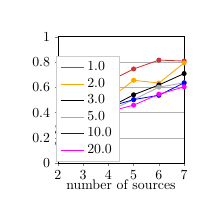
\begin{tikzpicture}

\definecolor{color0}{rgb}{0.8,0.207843137254902,0.219607843137255}
\definecolor{color1}{rgb}{1,0.647058823529412,0}
\definecolor{color2}{rgb}{1,0,1}

\begin{axis}[
title={err-mean},
xlabel={number of sources},
xmin=2, xmax=7,
ymin=0, ymax=1,
width=\figurewidth,
height=\figureheight,
tick align=outside,
tick pos=left,
x grid style={lightgray!92.026143790849673!black},
ymajorgrids,
y grid style={lightgray!92.026143790849673!black},
legend entries={{1.0},{2.0},{3.0},{5.0},{10.0},{20.0}},
legend style={at={(0.97,0.03)}, anchor=south east, draw=white!80.0!black},
legend cell align={left}
]
\addlegendimage{no markers, color0}
\addlegendimage{no markers, color1}
\addlegendimage{no markers, black}
\addlegendimage{no markers, lightgray!88.366013071895424!black}
\addlegendimage{no markers, blue}
\addlegendimage{no markers, color2}
\addplot [semithick, color0, mark=*, mark size=3, mark options={solid}]
table {%
2 0.290719260974231
3 0.479301880051738
4 0.644171288750938
5 0.744992267692781
6 0.815194102350153
7 0.80761917101706
};
\addplot [semithick, color1, mark=*, mark size=3, mark options={solid}]
table {%
2 0.245694149597362
3 0.421649843327725
4 0.500562120786198
5 0.655687681534857
6 0.633687481891525
7 0.793106398964979
};
\addplot [semithick, black, mark=*, mark size=3, mark options={solid}]
table {%
2 0.244192685094324
3 0.318939976510832
4 0.436516755504563
5 0.540639551860509
6 0.618377832825832
7 0.708533647793283
};
\addplot [semithick, lightgray!88.366013071895424!black, mark=*, mark size=3, mark options={solid}]
table {%
2 0.151357304870224
3 0.298658572932984
4 0.409077232118482
5 0.502185647164528
6 0.601037546098582
7 0.635845669023758
};
\addplot [semithick, blue, mark=*, mark size=3, mark options={solid}]
table {%
2 0.156145785073103
3 0.262900994349871
4 0.444291990749065
5 0.502497456459568
6 0.536465373800886
7 0.635142635271785
};
\addplot [semithick, color2, mark=*, mark size=3, mark options={solid}]
table {%
2 0.158641822221236
3 0.292719119608
4 0.407112096408886
5 0.458557818271804
6 0.545724599411615
7 0.603303151192354
};
\end{axis}

\end{tikzpicture}
	\end{subfigure}
    \begin{subfigure}{0.49\textwidth}
          \centering
	       \includestandalone[width=\textwidth]{data/plots/plot_em-iterations_percent-matched}
%            % This file was created by matplotlib2tikz v0.6.13.
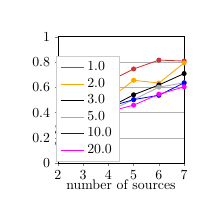
\begin{tikzpicture}

\definecolor{color0}{rgb}{0.8,0.207843137254902,0.219607843137255}
\definecolor{color1}{rgb}{1,0.647058823529412,0}
\definecolor{color2}{rgb}{1,0,1}

\begin{axis}[
title={err-mean},
xlabel={number of sources},
xmin=2, xmax=7,
ymin=0, ymax=1,
width=\figurewidth,
height=\figureheight,
tick align=outside,
tick pos=left,
x grid style={lightgray!92.026143790849673!black},
ymajorgrids,
y grid style={lightgray!92.026143790849673!black},
legend entries={{1.0},{2.0},{3.0},{5.0},{10.0},{20.0}},
legend style={at={(0.97,0.03)}, anchor=south east, draw=white!80.0!black},
legend cell align={left}
]
\addlegendimage{no markers, color0}
\addlegendimage{no markers, color1}
\addlegendimage{no markers, black}
\addlegendimage{no markers, lightgray!88.366013071895424!black}
\addlegendimage{no markers, blue}
\addlegendimage{no markers, color2}
\addplot [semithick, color0, mark=*, mark size=3, mark options={solid}]
table {%
2 0.290719260974231
3 0.479301880051738
4 0.644171288750938
5 0.744992267692781
6 0.815194102350153
7 0.80761917101706
};
\addplot [semithick, color1, mark=*, mark size=3, mark options={solid}]
table {%
2 0.245694149597362
3 0.421649843327725
4 0.500562120786198
5 0.655687681534857
6 0.633687481891525
7 0.793106398964979
};
\addplot [semithick, black, mark=*, mark size=3, mark options={solid}]
table {%
2 0.244192685094324
3 0.318939976510832
4 0.436516755504563
5 0.540639551860509
6 0.618377832825832
7 0.708533647793283
};
\addplot [semithick, lightgray!88.366013071895424!black, mark=*, mark size=3, mark options={solid}]
table {%
2 0.151357304870224
3 0.298658572932984
4 0.409077232118482
5 0.502185647164528
6 0.601037546098582
7 0.635845669023758
};
\addplot [semithick, blue, mark=*, mark size=3, mark options={solid}]
table {%
2 0.156145785073103
3 0.262900994349871
4 0.444291990749065
5 0.502497456459568
6 0.536465373800886
7 0.635142635271785
};
\addplot [semithick, color2, mark=*, mark size=3, mark options={solid}]
table {%
2 0.158641822221236
3 0.292719119608
4 0.407112096408886
5 0.458557818271804
6 0.545724599411615
7 0.603303151192354
};
\end{axis}

\end{tikzpicture}
	\end{subfigure}
\caption{Evaluation of EM-Iterations (T60=0.6, SNR=0, refl-ord=3, n=150)}
\end{figure}

\begin{itemize}
\item Not surprising, more iterations mean less estimation error and more matched sources
\item 1 and 2 iterations have considerable worse performance
\item from 3 on, performance seems to be stable
\item no difference between 10 and 20
\item Therefore, Future trials with em=5
\end{itemize}

\subsection*{T60}
\begin{figure}[H]
    \centering
    \begin{subfigure}{0.49\textwidth}
          \centering
	       \includestandalone[width=\textwidth]{data/plots/plot_T60_err-mean}
%            % This file was created by matplotlib2tikz v0.6.13.
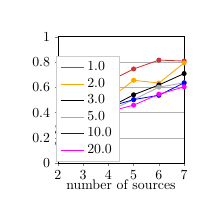
\begin{tikzpicture}

\definecolor{color0}{rgb}{0.8,0.207843137254902,0.219607843137255}
\definecolor{color1}{rgb}{1,0.647058823529412,0}
\definecolor{color2}{rgb}{1,0,1}

\begin{axis}[
title={err-mean},
xlabel={number of sources},
xmin=2, xmax=7,
ymin=0, ymax=1,
width=\figurewidth,
height=\figureheight,
tick align=outside,
tick pos=left,
x grid style={lightgray!92.026143790849673!black},
ymajorgrids,
y grid style={lightgray!92.026143790849673!black},
legend entries={{1.0},{2.0},{3.0},{5.0},{10.0},{20.0}},
legend style={at={(0.97,0.03)}, anchor=south east, draw=white!80.0!black},
legend cell align={left}
]
\addlegendimage{no markers, color0}
\addlegendimage{no markers, color1}
\addlegendimage{no markers, black}
\addlegendimage{no markers, lightgray!88.366013071895424!black}
\addlegendimage{no markers, blue}
\addlegendimage{no markers, color2}
\addplot [semithick, color0, mark=*, mark size=3, mark options={solid}]
table {%
2 0.290719260974231
3 0.479301880051738
4 0.644171288750938
5 0.744992267692781
6 0.815194102350153
7 0.80761917101706
};
\addplot [semithick, color1, mark=*, mark size=3, mark options={solid}]
table {%
2 0.245694149597362
3 0.421649843327725
4 0.500562120786198
5 0.655687681534857
6 0.633687481891525
7 0.793106398964979
};
\addplot [semithick, black, mark=*, mark size=3, mark options={solid}]
table {%
2 0.244192685094324
3 0.318939976510832
4 0.436516755504563
5 0.540639551860509
6 0.618377832825832
7 0.708533647793283
};
\addplot [semithick, lightgray!88.366013071895424!black, mark=*, mark size=3, mark options={solid}]
table {%
2 0.151357304870224
3 0.298658572932984
4 0.409077232118482
5 0.502185647164528
6 0.601037546098582
7 0.635845669023758
};
\addplot [semithick, blue, mark=*, mark size=3, mark options={solid}]
table {%
2 0.156145785073103
3 0.262900994349871
4 0.444291990749065
5 0.502497456459568
6 0.536465373800886
7 0.635142635271785
};
\addplot [semithick, color2, mark=*, mark size=3, mark options={solid}]
table {%
2 0.158641822221236
3 0.292719119608
4 0.407112096408886
5 0.458557818271804
6 0.545724599411615
7 0.603303151192354
};
\end{axis}

\end{tikzpicture}
	\end{subfigure}
    \begin{subfigure}{0.49\textwidth}
          \centering
	       \includestandalone[width=\textwidth]{data/plots/plot_T60_percent-matched}
%            % This file was created by matplotlib2tikz v0.6.13.
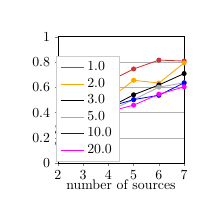
\begin{tikzpicture}

\definecolor{color0}{rgb}{0.8,0.207843137254902,0.219607843137255}
\definecolor{color1}{rgb}{1,0.647058823529412,0}
\definecolor{color2}{rgb}{1,0,1}

\begin{axis}[
title={err-mean},
xlabel={number of sources},
xmin=2, xmax=7,
ymin=0, ymax=1,
width=\figurewidth,
height=\figureheight,
tick align=outside,
tick pos=left,
x grid style={lightgray!92.026143790849673!black},
ymajorgrids,
y grid style={lightgray!92.026143790849673!black},
legend entries={{1.0},{2.0},{3.0},{5.0},{10.0},{20.0}},
legend style={at={(0.97,0.03)}, anchor=south east, draw=white!80.0!black},
legend cell align={left}
]
\addlegendimage{no markers, color0}
\addlegendimage{no markers, color1}
\addlegendimage{no markers, black}
\addlegendimage{no markers, lightgray!88.366013071895424!black}
\addlegendimage{no markers, blue}
\addlegendimage{no markers, color2}
\addplot [semithick, color0, mark=*, mark size=3, mark options={solid}]
table {%
2 0.290719260974231
3 0.479301880051738
4 0.644171288750938
5 0.744992267692781
6 0.815194102350153
7 0.80761917101706
};
\addplot [semithick, color1, mark=*, mark size=3, mark options={solid}]
table {%
2 0.245694149597362
3 0.421649843327725
4 0.500562120786198
5 0.655687681534857
6 0.633687481891525
7 0.793106398964979
};
\addplot [semithick, black, mark=*, mark size=3, mark options={solid}]
table {%
2 0.244192685094324
3 0.318939976510832
4 0.436516755504563
5 0.540639551860509
6 0.618377832825832
7 0.708533647793283
};
\addplot [semithick, lightgray!88.366013071895424!black, mark=*, mark size=3, mark options={solid}]
table {%
2 0.151357304870224
3 0.298658572932984
4 0.409077232118482
5 0.502185647164528
6 0.601037546098582
7 0.635845669023758
};
\addplot [semithick, blue, mark=*, mark size=3, mark options={solid}]
table {%
2 0.156145785073103
3 0.262900994349871
4 0.444291990749065
5 0.502497456459568
6 0.536465373800886
7 0.635142635271785
};
\addplot [semithick, color2, mark=*, mark size=3, mark options={solid}]
table {%
2 0.158641822221236
3 0.292719119608
4 0.407112096408886
5 0.458557818271804
6 0.545724599411615
7 0.603303151192354
};
\end{axis}

\end{tikzpicture}
	\end{subfigure}
\caption{Evaluation of T60 (EM-Iterations=10, SNR=0, refl-ord=-1, n=100)}
\end{figure}

\subsection*{Reflect Order}
%\begin{figure}[H]
%    \centering
%    \begin{subfigure}{0.49\textwidth}
%          \centering
%	       \includestandalone[width=\textwidth]{data/plots/plot_reflect-order_err-mean}
%%            % This file was created by matplotlib2tikz v0.6.13.
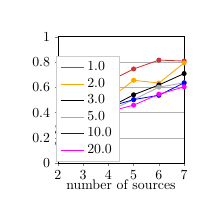
\begin{tikzpicture}

\definecolor{color0}{rgb}{0.8,0.207843137254902,0.219607843137255}
\definecolor{color1}{rgb}{1,0.647058823529412,0}
\definecolor{color2}{rgb}{1,0,1}

\begin{axis}[
title={err-mean},
xlabel={number of sources},
xmin=2, xmax=7,
ymin=0, ymax=1,
width=\figurewidth,
height=\figureheight,
tick align=outside,
tick pos=left,
x grid style={lightgray!92.026143790849673!black},
ymajorgrids,
y grid style={lightgray!92.026143790849673!black},
legend entries={{1.0},{2.0},{3.0},{5.0},{10.0},{20.0}},
legend style={at={(0.97,0.03)}, anchor=south east, draw=white!80.0!black},
legend cell align={left}
]
\addlegendimage{no markers, color0}
\addlegendimage{no markers, color1}
\addlegendimage{no markers, black}
\addlegendimage{no markers, lightgray!88.366013071895424!black}
\addlegendimage{no markers, blue}
\addlegendimage{no markers, color2}
\addplot [semithick, color0, mark=*, mark size=3, mark options={solid}]
table {%
2 0.290719260974231
3 0.479301880051738
4 0.644171288750938
5 0.744992267692781
6 0.815194102350153
7 0.80761917101706
};
\addplot [semithick, color1, mark=*, mark size=3, mark options={solid}]
table {%
2 0.245694149597362
3 0.421649843327725
4 0.500562120786198
5 0.655687681534857
6 0.633687481891525
7 0.793106398964979
};
\addplot [semithick, black, mark=*, mark size=3, mark options={solid}]
table {%
2 0.244192685094324
3 0.318939976510832
4 0.436516755504563
5 0.540639551860509
6 0.618377832825832
7 0.708533647793283
};
\addplot [semithick, lightgray!88.366013071895424!black, mark=*, mark size=3, mark options={solid}]
table {%
2 0.151357304870224
3 0.298658572932984
4 0.409077232118482
5 0.502185647164528
6 0.601037546098582
7 0.635845669023758
};
\addplot [semithick, blue, mark=*, mark size=3, mark options={solid}]
table {%
2 0.156145785073103
3 0.262900994349871
4 0.444291990749065
5 0.502497456459568
6 0.536465373800886
7 0.635142635271785
};
\addplot [semithick, color2, mark=*, mark size=3, mark options={solid}]
table {%
2 0.158641822221236
3 0.292719119608
4 0.407112096408886
5 0.458557818271804
6 0.545724599411615
7 0.603303151192354
};
\end{axis}

\end{tikzpicture}
%	\end{subfigure}
%    \begin{subfigure}{0.49\textwidth}
%          \centering
%	       \includestandalone[width=\textwidth]{data/plots/plot_reflect-order_percent-matched}
%%            % This file was created by matplotlib2tikz v0.6.13.
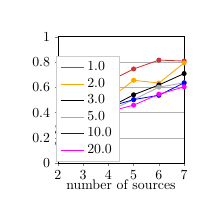
\begin{tikzpicture}

\definecolor{color0}{rgb}{0.8,0.207843137254902,0.219607843137255}
\definecolor{color1}{rgb}{1,0.647058823529412,0}
\definecolor{color2}{rgb}{1,0,1}

\begin{axis}[
title={err-mean},
xlabel={number of sources},
xmin=2, xmax=7,
ymin=0, ymax=1,
width=\figurewidth,
height=\figureheight,
tick align=outside,
tick pos=left,
x grid style={lightgray!92.026143790849673!black},
ymajorgrids,
y grid style={lightgray!92.026143790849673!black},
legend entries={{1.0},{2.0},{3.0},{5.0},{10.0},{20.0}},
legend style={at={(0.97,0.03)}, anchor=south east, draw=white!80.0!black},
legend cell align={left}
]
\addlegendimage{no markers, color0}
\addlegendimage{no markers, color1}
\addlegendimage{no markers, black}
\addlegendimage{no markers, lightgray!88.366013071895424!black}
\addlegendimage{no markers, blue}
\addlegendimage{no markers, color2}
\addplot [semithick, color0, mark=*, mark size=3, mark options={solid}]
table {%
2 0.290719260974231
3 0.479301880051738
4 0.644171288750938
5 0.744992267692781
6 0.815194102350153
7 0.80761917101706
};
\addplot [semithick, color1, mark=*, mark size=3, mark options={solid}]
table {%
2 0.245694149597362
3 0.421649843327725
4 0.500562120786198
5 0.655687681534857
6 0.633687481891525
7 0.793106398964979
};
\addplot [semithick, black, mark=*, mark size=3, mark options={solid}]
table {%
2 0.244192685094324
3 0.318939976510832
4 0.436516755504563
5 0.540639551860509
6 0.618377832825832
7 0.708533647793283
};
\addplot [semithick, lightgray!88.366013071895424!black, mark=*, mark size=3, mark options={solid}]
table {%
2 0.151357304870224
3 0.298658572932984
4 0.409077232118482
5 0.502185647164528
6 0.601037546098582
7 0.635845669023758
};
\addplot [semithick, blue, mark=*, mark size=3, mark options={solid}]
table {%
2 0.156145785073103
3 0.262900994349871
4 0.444291990749065
5 0.502497456459568
6 0.536465373800886
7 0.635142635271785
};
\addplot [semithick, color2, mark=*, mark size=3, mark options={solid}]
table {%
2 0.158641822221236
3 0.292719119608
4 0.407112096408886
5 0.458557818271804
6 0.545724599411615
7 0.603303151192354
};
\end{axis}

\end{tikzpicture}
%	\end{subfigure}
%\caption{Evaluation of Reflect Order (EM-Iterations=5, T60=0.6, SNR=0, n=250)}
%\end{figure}

\subsection*{SNR}
\begin{figure}[H]
    \centering
    \begin{subfigure}{0.49\textwidth}
          \centering
	       \includestandalone[width=\textwidth]{data/plots/plot_snr_err-mean}
%            % This file was created by matplotlib2tikz v0.6.13.
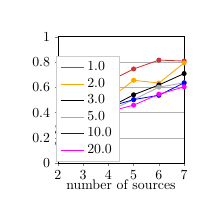
\begin{tikzpicture}

\definecolor{color0}{rgb}{0.8,0.207843137254902,0.219607843137255}
\definecolor{color1}{rgb}{1,0.647058823529412,0}
\definecolor{color2}{rgb}{1,0,1}

\begin{axis}[
title={err-mean},
xlabel={number of sources},
xmin=2, xmax=7,
ymin=0, ymax=1,
width=\figurewidth,
height=\figureheight,
tick align=outside,
tick pos=left,
x grid style={lightgray!92.026143790849673!black},
ymajorgrids,
y grid style={lightgray!92.026143790849673!black},
legend entries={{1.0},{2.0},{3.0},{5.0},{10.0},{20.0}},
legend style={at={(0.97,0.03)}, anchor=south east, draw=white!80.0!black},
legend cell align={left}
]
\addlegendimage{no markers, color0}
\addlegendimage{no markers, color1}
\addlegendimage{no markers, black}
\addlegendimage{no markers, lightgray!88.366013071895424!black}
\addlegendimage{no markers, blue}
\addlegendimage{no markers, color2}
\addplot [semithick, color0, mark=*, mark size=3, mark options={solid}]
table {%
2 0.290719260974231
3 0.479301880051738
4 0.644171288750938
5 0.744992267692781
6 0.815194102350153
7 0.80761917101706
};
\addplot [semithick, color1, mark=*, mark size=3, mark options={solid}]
table {%
2 0.245694149597362
3 0.421649843327725
4 0.500562120786198
5 0.655687681534857
6 0.633687481891525
7 0.793106398964979
};
\addplot [semithick, black, mark=*, mark size=3, mark options={solid}]
table {%
2 0.244192685094324
3 0.318939976510832
4 0.436516755504563
5 0.540639551860509
6 0.618377832825832
7 0.708533647793283
};
\addplot [semithick, lightgray!88.366013071895424!black, mark=*, mark size=3, mark options={solid}]
table {%
2 0.151357304870224
3 0.298658572932984
4 0.409077232118482
5 0.502185647164528
6 0.601037546098582
7 0.635845669023758
};
\addplot [semithick, blue, mark=*, mark size=3, mark options={solid}]
table {%
2 0.156145785073103
3 0.262900994349871
4 0.444291990749065
5 0.502497456459568
6 0.536465373800886
7 0.635142635271785
};
\addplot [semithick, color2, mark=*, mark size=3, mark options={solid}]
table {%
2 0.158641822221236
3 0.292719119608
4 0.407112096408886
5 0.458557818271804
6 0.545724599411615
7 0.603303151192354
};
\end{axis}

\end{tikzpicture}
	\end{subfigure}
    \begin{subfigure}{0.49\textwidth}
          \centering
	       \includestandalone[width=\textwidth]{data/plots/plot_snr_percent-matched}
%            % This file was created by matplotlib2tikz v0.6.13.
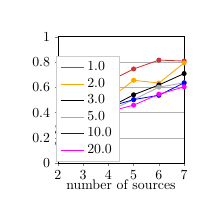
\begin{tikzpicture}

\definecolor{color0}{rgb}{0.8,0.207843137254902,0.219607843137255}
\definecolor{color1}{rgb}{1,0.647058823529412,0}
\definecolor{color2}{rgb}{1,0,1}

\begin{axis}[
title={err-mean},
xlabel={number of sources},
xmin=2, xmax=7,
ymin=0, ymax=1,
width=\figurewidth,
height=\figureheight,
tick align=outside,
tick pos=left,
x grid style={lightgray!92.026143790849673!black},
ymajorgrids,
y grid style={lightgray!92.026143790849673!black},
legend entries={{1.0},{2.0},{3.0},{5.0},{10.0},{20.0}},
legend style={at={(0.97,0.03)}, anchor=south east, draw=white!80.0!black},
legend cell align={left}
]
\addlegendimage{no markers, color0}
\addlegendimage{no markers, color1}
\addlegendimage{no markers, black}
\addlegendimage{no markers, lightgray!88.366013071895424!black}
\addlegendimage{no markers, blue}
\addlegendimage{no markers, color2}
\addplot [semithick, color0, mark=*, mark size=3, mark options={solid}]
table {%
2 0.290719260974231
3 0.479301880051738
4 0.644171288750938
5 0.744992267692781
6 0.815194102350153
7 0.80761917101706
};
\addplot [semithick, color1, mark=*, mark size=3, mark options={solid}]
table {%
2 0.245694149597362
3 0.421649843327725
4 0.500562120786198
5 0.655687681534857
6 0.633687481891525
7 0.793106398964979
};
\addplot [semithick, black, mark=*, mark size=3, mark options={solid}]
table {%
2 0.244192685094324
3 0.318939976510832
4 0.436516755504563
5 0.540639551860509
6 0.618377832825832
7 0.708533647793283
};
\addplot [semithick, lightgray!88.366013071895424!black, mark=*, mark size=3, mark options={solid}]
table {%
2 0.151357304870224
3 0.298658572932984
4 0.409077232118482
5 0.502185647164528
6 0.601037546098582
7 0.635845669023758
};
\addplot [semithick, blue, mark=*, mark size=3, mark options={solid}]
table {%
2 0.156145785073103
3 0.262900994349871
4 0.444291990749065
5 0.502497456459568
6 0.536465373800886
7 0.635142635271785
};
\addplot [semithick, color2, mark=*, mark size=3, mark options={solid}]
table {%
2 0.158641822221236
3 0.292719119608
4 0.407112096408886
5 0.458557818271804
6 0.545724599411615
7 0.603303151192354
};
\end{axis}

\end{tikzpicture}
	\end{subfigure}
\caption{Evaluation of SNR (EM-Iterations=5, T60=0.3, refl-ord=3, n=200)}
\end{figure}

%\input{chapters/5results/source_tracking}
\chapter{Conclusions}                       \label{chap:concl}

\section{Critical review}   
\begin{itemize}
    \item Implementation
    \begin{itemize}
        \item Mix signals in STFT-Domain directly, instead of calculating $Y*X$ in the STFT-Domain, transforming back into time-domain to mix signals only to transform back into STFT domain for PRP calculation.
        \item Fixed mean, fixed variance: Is this really the best model for this problem?
        \item Could remove reliance on gridpoints by also estimating mean and only having $S$ Gaussian components instead of $T\cdot K\cdot |\mathcal{P}|$
    \end{itemize}
\end{itemize}

\section{Further research}
%\input{chapters/6conclusion/further_research}



%\chapter[Testbed]{Testbed}
\chaptermark{Testbed}
\label{chap:Testbed}
This is a section, where LaTeX functionality can be tested!
\section{Graphics}
\subsection{Including .eps-files}

\begin{figure}[H]
\centering
\includegraphics[width=0.5\textwidth]{static/gaussian}
\caption{Multiple three-dimensional gaussian distributions...}
\label{fig:mog}
\end{figure}


This is the text beneath an included picture. Figure \ref{fig:mog} shows an example of how to include eps-figures in this document.

\subsection{Including tikz-figures}
Graphs can be included, like is shown in figure \ref{fig:sin}, using the input-method.
\tikzset{every picture/.style={scale=0.9}}
\begin{figure}[H]
	\centering
	% This file was created by matlab2tikz.
%
%The latest updates can be retrieved from
%  http://www.mathworks.com/matlabcentral/fileexchange/22022-matlab2tikz-matlab2tikz
%where you can also make suggestions and rate matlab2tikz.
%
\definecolor{mycolor1}{rgb}{0.00000,0.44700,0.74100}%
%
\begin{tikzpicture}

\begin{axis}[%
width=6.028in,
height=4.754in,
at={(1.011in,0.642in)},
scale only axis,
xmin=0,
xmax=6.28318530717959,
xtick={0,1.5707963267949,3.14159265358979,4.71238898038469,6.28318530717959},
xticklabels={{0},{$\text{1/2 }\pi$},{$\pi$},{$\text{3/2 }\pi$},{$\text{2}\pi$}},
ymin=-1.5,
ymax=1.5,
ytick={-1,  0,  1},
axis background/.style={fill=white}
]
\addplot [color=mycolor1, forget plot]
  table[row sep=crcr]{%
0	0\\
0.126933036508679	0.126592453573749\\
0.253866073017357	0.251147987181079\\
0.380799109526036	0.371662455660328\\
0.507732146034714	0.486196736100469\\
0.634665182543393	0.59290792905464\\
0.761598219052071	0.690079011482112\\
0.88853125556075	0.776146464291757\\
1.01546429206943	0.849725429949514\\
1.14239732857811	0.909631995354518\\
1.26933036508679	0.954902241444074\\
1.39626340159546	0.984807753012208\\
1.52319643810414	0.998867339183008\\
1.65012947461282	0.996854775951942\\
1.7770625111215	0.978802446214779\\
1.90399554763018	0.945000818714669\\
2.03092858413886	0.895993774291336\\
2.15786162064753	0.832569854634771\\
2.28479465715621	0.755749574354258\\
2.41172769366489	0.666769000516292\\
2.53866073017357	0.567059863862771\\
2.66559376668225	0.458226521727411\\
2.79252680319093	0.342020143325669\\
2.91945983969961	0.220310532786541\\
3.04639287620828	0.0950560433041829\\
3.17332591271696	-0.0317279334980679\\
3.30025894922564	-0.15800139597335\\
3.42719198573432	-0.281732556841429\\
3.554125022243	-0.400930535406613\\
3.68105805875168	-0.513677391573406\\
3.80799109526036	-0.618158986220605\\
3.93492413176903	-0.712694171378863\\
4.06185716827771	-0.795761840530832\\
4.18879020478639	-0.866025403784438\\
4.31572324129507	-0.922354294104581\\
4.44265627780375	-0.963842158559942\\
4.56958931431243	-0.989821441880933\\
4.69652235082111	-0.999874127673875\\
4.82345538732978	-0.993838464461254\\
4.95038842383846	-0.971811568323542\\
5.07732146034714	-0.934147860265107\\
5.20425449685582	-0.881453363447582\\
5.3311875333645	-0.814575952050336\\
5.45812056987318	-0.734591708657534\\
5.58505360638185	-0.64278760968654\\
5.71198664289053	-0.540640817455597\\
5.83891967939921	-0.429794912089172\\
5.96585271590789	-0.312033445698487\\
6.09278575241657	-0.189251244360411\\
6.21971878892525	-0.0634239196565654\\
6.34665182543393	0.0634239196565649\\
6.4735848619426	0.18925124436041\\
6.60051789845128	0.312033445698487\\
6.72745093495996	0.429794912089172\\
6.85438397146864	0.540640817455597\\
6.98131700797732	0.642787609686539\\
7.108250044486	0.734591708657533\\
7.23518308099467	0.814575952050335\\
7.36211611750335	0.881453363447582\\
7.48904915401203	0.934147860265107\\
7.61598219052071	0.971811568323542\\
7.74291522702939	0.993838464461254\\
7.86984826353807	0.999874127673875\\
7.99678130004675	0.989821441880933\\
8.12371433655542	0.963842158559942\\
8.2506473730641	0.922354294104582\\
8.37758040957278	0.866025403784439\\
8.50451344608146	0.795761840530832\\
8.63144648259014	0.712694171378863\\
8.75837951909882	0.618158986220606\\
8.88531255560749	0.513677391573407\\
9.01224559211617	0.400930535406613\\
9.13917862862485	0.28173255684143\\
9.26611166513353	0.158001395973351\\
9.39304470164221	0.031727933498067\\
9.51997773815089	-0.0950560433041828\\
9.64691077465957	-0.22031053278654\\
9.77384381116824	-0.342020143325668\\
9.90077684767692	-0.458226521727409\\
10.0277098841856	-0.567059863862771\\
10.1546429206943	-0.666769000516291\\
10.281575957203	-0.755749574354258\\
10.4085089937116	-0.832569854634771\\
10.5354420302203	-0.895993774291336\\
10.662375066729	-0.945000818714668\\
10.7893081032377	-0.978802446214779\\
10.9162411397464	-0.996854775951942\\
11.043174176255	-0.998867339183008\\
11.1701072127637	-0.984807753012208\\
11.2970402492724	-0.954902241444074\\
11.4239732857811	-0.909631995354518\\
11.5509063222897	-0.849725429949514\\
11.6778393587984	-0.776146464291757\\
11.8047723953071	-0.690079011482113\\
11.9317054318158	-0.59290792905464\\
12.0586384683245	-0.486196736100469\\
12.1855715048331	-0.371662455660328\\
12.3125045413418	-0.251147987181081\\
12.4394375778505	-0.126592453573751\\
12.5663706143592	-4.89858719658941e-16\\
};
\end{axis}
\end{tikzpicture}%
	\caption{A sine wave}
	\label{fig:sin}
\end{figure}

As figure \ref{fig:sin} was a little big, we now try to scale this output somehow:

\tikzset{every picture/.style={scale=0.6}}
\begin{figure}[H]
	\centering
	% This file was created by matlab2tikz.
%
%The latest updates can be retrieved from
%  http://www.mathworks.com/matlabcentral/fileexchange/22022-matlab2tikz-matlab2tikz
%where you can also make suggestions and rate matlab2tikz.
%
\definecolor{mycolor1}{rgb}{0.00000,0.44700,0.74100}%
%
\begin{tikzpicture}

\begin{axis}[%
width=6.028in,
height=4.754in,
at={(1.011in,0.642in)},
scale only axis,
xmin=0,
xmax=6.28318530717959,
xtick={0,1.5707963267949,3.14159265358979,4.71238898038469,6.28318530717959},
xticklabels={{0},{$\text{1/2 }\pi$},{$\pi$},{$\text{3/2 }\pi$},{$\text{2}\pi$}},
ymin=-1.5,
ymax=1.5,
ytick={-1,  0,  1},
axis background/.style={fill=white}
]
\addplot [color=mycolor1, forget plot]
  table[row sep=crcr]{%
0	0\\
0.126933036508679	0.126592453573749\\
0.253866073017357	0.251147987181079\\
0.380799109526036	0.371662455660328\\
0.507732146034714	0.486196736100469\\
0.634665182543393	0.59290792905464\\
0.761598219052071	0.690079011482112\\
0.88853125556075	0.776146464291757\\
1.01546429206943	0.849725429949514\\
1.14239732857811	0.909631995354518\\
1.26933036508679	0.954902241444074\\
1.39626340159546	0.984807753012208\\
1.52319643810414	0.998867339183008\\
1.65012947461282	0.996854775951942\\
1.7770625111215	0.978802446214779\\
1.90399554763018	0.945000818714669\\
2.03092858413886	0.895993774291336\\
2.15786162064753	0.832569854634771\\
2.28479465715621	0.755749574354258\\
2.41172769366489	0.666769000516292\\
2.53866073017357	0.567059863862771\\
2.66559376668225	0.458226521727411\\
2.79252680319093	0.342020143325669\\
2.91945983969961	0.220310532786541\\
3.04639287620828	0.0950560433041829\\
3.17332591271696	-0.0317279334980679\\
3.30025894922564	-0.15800139597335\\
3.42719198573432	-0.281732556841429\\
3.554125022243	-0.400930535406613\\
3.68105805875168	-0.513677391573406\\
3.80799109526036	-0.618158986220605\\
3.93492413176903	-0.712694171378863\\
4.06185716827771	-0.795761840530832\\
4.18879020478639	-0.866025403784438\\
4.31572324129507	-0.922354294104581\\
4.44265627780375	-0.963842158559942\\
4.56958931431243	-0.989821441880933\\
4.69652235082111	-0.999874127673875\\
4.82345538732978	-0.993838464461254\\
4.95038842383846	-0.971811568323542\\
5.07732146034714	-0.934147860265107\\
5.20425449685582	-0.881453363447582\\
5.3311875333645	-0.814575952050336\\
5.45812056987318	-0.734591708657534\\
5.58505360638185	-0.64278760968654\\
5.71198664289053	-0.540640817455597\\
5.83891967939921	-0.429794912089172\\
5.96585271590789	-0.312033445698487\\
6.09278575241657	-0.189251244360411\\
6.21971878892525	-0.0634239196565654\\
6.34665182543393	0.0634239196565649\\
6.4735848619426	0.18925124436041\\
6.60051789845128	0.312033445698487\\
6.72745093495996	0.429794912089172\\
6.85438397146864	0.540640817455597\\
6.98131700797732	0.642787609686539\\
7.108250044486	0.734591708657533\\
7.23518308099467	0.814575952050335\\
7.36211611750335	0.881453363447582\\
7.48904915401203	0.934147860265107\\
7.61598219052071	0.971811568323542\\
7.74291522702939	0.993838464461254\\
7.86984826353807	0.999874127673875\\
7.99678130004675	0.989821441880933\\
8.12371433655542	0.963842158559942\\
8.2506473730641	0.922354294104582\\
8.37758040957278	0.866025403784439\\
8.50451344608146	0.795761840530832\\
8.63144648259014	0.712694171378863\\
8.75837951909882	0.618158986220606\\
8.88531255560749	0.513677391573407\\
9.01224559211617	0.400930535406613\\
9.13917862862485	0.28173255684143\\
9.26611166513353	0.158001395973351\\
9.39304470164221	0.031727933498067\\
9.51997773815089	-0.0950560433041828\\
9.64691077465957	-0.22031053278654\\
9.77384381116824	-0.342020143325668\\
9.90077684767692	-0.458226521727409\\
10.0277098841856	-0.567059863862771\\
10.1546429206943	-0.666769000516291\\
10.281575957203	-0.755749574354258\\
10.4085089937116	-0.832569854634771\\
10.5354420302203	-0.895993774291336\\
10.662375066729	-0.945000818714668\\
10.7893081032377	-0.978802446214779\\
10.9162411397464	-0.996854775951942\\
11.043174176255	-0.998867339183008\\
11.1701072127637	-0.984807753012208\\
11.2970402492724	-0.954902241444074\\
11.4239732857811	-0.909631995354518\\
11.5509063222897	-0.849725429949514\\
11.6778393587984	-0.776146464291757\\
11.8047723953071	-0.690079011482113\\
11.9317054318158	-0.59290792905464\\
12.0586384683245	-0.486196736100469\\
12.1855715048331	-0.371662455660328\\
12.3125045413418	-0.251147987181081\\
12.4394375778505	-0.126592453573751\\
12.5663706143592	-4.89858719658941e-16\\
};
\end{axis}
\end{tikzpicture}%
	\caption{A second sine wave}
	\label{fig:sin2}
\end{figure}

But, in doing this, scaling the tikz output might not be as easy as with the includegraphics-method. This is where the standalone package comes in handy.

\subsection{Grouping plots on page}
\subsubsection{2 tikz-figures}
\tikzset{every picture/.style={scale=0.5}}
\begin{figure}[H]
	\centering
	\begin{subfigure}{0.49\textwidth}
		\includestandalone[width=\textwidth]{plots/static/sin-tikz}
		\caption{A sine wave}
	\end{subfigure}
	\begin{subfigure}{0.49\textwidth}
		\includestandalone[width=\textwidth]{plots/static/cos-tikz}
		\caption{A cosine wave}
	\end{subfigure}
	\caption{Sine and cosine waves}
	\label{fig:sin}
\end{figure}

\subsubsection{2 .eps figures}
\begin{figure}[H]
 \centering
 \begin{subfigure}{0.49\textwidth}
    \includegraphics[width=\textwidth]{gaussian}
    \caption{Sub caption}
 \end{subfigure}
 \begin{subfigure}{0.49\textwidth}
    \includegraphics[width=\textwidth]{gaussian}
    \caption{Sub caption}
 \end{subfigure}
 \caption{Main caption}
\end{figure}

\newpage
\section{Citations}
\subsection{Simple Citations}
The EM-Algorithm is covered in depth by Bishop "EM algorithm, is a general technique for finding maximum likelihood solutions for probabilistic models having latent variables (Dempster et al., 1977; McLachlan and Krishnan, 1997). \cite[p. 472]{Bishop2006}. Reverberant environments, secondary reflections, may result in biased location estimates \cite[p.1]{Schwartz2014}
%\chapter{Chapter}
\section{Section}
\subsection{Subsection}
\subsubsection{Subsubsection}
\paragraph{Paragraph}
\subparagraph{Subparagraph}


%%%%%%%%%%%%%%%%%%%%%%%%%%%%%%%%  D O C U M E N T  %%%%%%%%%%%%%%%%%%%%%%%%%%%%%%%%%
%%%%%%%%%%%%%%%%%%%%%%%%%%%%%%%%%%%%%%%%%%%%%%%%%%%%%%%%%%%%%%%%%%%%%%%%%%%%%%%%%%%%
%%%%%%%%%%%%%%%%%%%%%%%%%%%%%%%%  A P P E N D I X  %%%%%%%%%%%%%%%%%%%%%%%%%%%%%%%%%

% ANHANG
\appendix
	\renewcommand{\chaptermark}[1]{\markboth{\uppercase{Appendix \thechapter:\ #1}}{}}
%	\todos
	
	\chapter{Formulas}
	\section*{Arithmetic Rules}
% Don't include basic logarithm rules! Lowers level of detail for all other calculations...
%\begin{align}
%\label{eq:log-sum}
%\ln(x\cdot y)&=\ln(x)+\ln(y),\\
%\label{eq:log-power}
%\ln(x^r)&=r\cdot\ln(x).
%\end{align}

\section*{Definitions}
	\chapter{Code}
%	\section{\texorpdfstring{\matlab} Code}
\label{sec:appCode}
\subsection*{simulate.m}
%\lstinputlisting[firstline=16, lastline=60]{/Users/jannismainczyk/thesis/src/matlab/mainczjs/simulate.m}
    \chapter{Results}
%	\section{Evaluation results data}
\label{sec:appData}
\subsection*{2 sources}
\begin{table}[H]
	\centering
	\input{data/tables/2017-10-03-16-47-02_2s_0.5m_results}
	\caption{2 sources, 0.5m source-distance, 1.2m wall-distance}
\end{table}

\subsection*{3 sources}
\begin{table}[H]
	\centering
	\input{data/tables/2017-10-03-17-00-20_3s_0.5m_results}
	\caption{3 sources, 0.5m source-distance, 1.2m wall-distance}
\end{table}

\subsection*{4 sources}
\begin{table}[H]
	\centering
	\input{data/tables/2017-10-03-17-14-39_4s_0.5m_results}
	\caption{4 sources, 0.5m source-distance, 1.2m wall-distance}
\end{table}


%    \begin{algorithm}[H]
\caption{The \acrshort{crem} algorithm for the exponential family}
\label{alg:crem-general}
\begin{algorithmic}
\State \textbf{initialize} $\theta^{(0)}_R$
\For{$t=1$ \textbf{to} $T$}
\State \textbf{E-Step}
\begin{align*}
	\bar\eta(\phi_t,x_t)&=E\left\{\eta(\phi_t,x_t)\mid\phi_t;\theta_R^{(t-1)} \right\}\\
\eta^R(\phi_t,x_t)&=\eta^R(\phi_{t-1},x_{t-1})+\gamma_t\big(\bar\eta(\phi_t,x_t)-\eta^R(\phi_{t-1},x_{t-1})\big)\\
\intertext{\State\textbf{M-Step}}
\theta^{(t)}_R&=\arg \max_\theta\big\langle\eta^R(\phi_t,x_t),\xi(\theta)\big\rangle
\end{align*}\EndFor
\end{algorithmic}
\end{algorithm}
	
	\clearpage
	\newpage

% LIST OF FIGURES
\addcontentsline{toc}{chapter}{List of Figures}
\listoffigures

% LIST OF TABLES
\addcontentsline{toc}{chapter}{List of Tables}
\listoftables

% Glossary
\setglossarystyle{altlist}
\printglossary[title=Glossary]

% LITERATURVERZEICHNIS
%nicht referenzierte Literaturstellen
\nocite{*}
\printbibliography
%\newpage
%%Eintrag im Inhaltsverzeichnis
%\addtocounter{page}{1}
%\addcontentsline{toc}{chapter}{Literaturverzeichnis}
%\addtocounter{page}{-1}
